%%%%%%%%%%%%%%%%%%%%%%%%%%%%%%%%%%%
% run with $ pdflatex LjLabBook.tex
%%%%%%%%%%%%%%%%%%%%%%%%%%%%%%%%%%%

\documentclass[12pt]{cmspaper}
\usepackage{mathtools} % includes the "amsmath" package and other mathematical symbols and environments
\usepackage{amssymb} % for an extended library of mathematical symbols
\usepackage[ampersand]{easylist} % for bullet points and lists, etc. New entry starts with & character
\usepackage{hyperref}
\usepackage{textcomp}

\begin{document}
\begin{titlepage}
  \cmsnote{LjLabBook}
  \date{\today}
  \title{HOW TO 9+t $\Longrightarrow$ \bf{5+t}}
  \begin{Authlist}
    Joe Taylor
  \end{Authlist}
\end{titlepage}

\pagenumbering{roman} % use Roman numerals in contents pages
\hypersetup{
  colorlinks,
  citecolor=black,
  filecolor=black,
  linkcolor=black,
  urlcolor=black
}
\setcounter{secnumdepth}{2}
\setcounter{tocdepth}{2}
\tableofcontents % adds a contents page
\newpage
\pagenumbering{arabic} % change page numbering back to Arabic numbers

\section{Scikit-Learn}

Jupyter notebook examples can be found here: \textit{https://github.com/ageron/handson-ml2}\newline

%%%%%%%%%%%%%%%%%%%%%%%%%%%
%%%%%%%%%%%%%%%%%%%%%%%%%%%
%%%%%%%%%%%%%%%%%%%%%%%%%%%
%%%%%%%%%%%%%%%%%%%%%%%%%%%
%%%%%%%%%%%%%%%%%%%%%%%%%%%
\subsection{Introduction}

\underline{What is Machine Learning?}
\begin{itemize}
\vspace{-4.0mm}
\item
ML is about making machines get better at some task by learning from data,
instead of having to explicitly code rules.
\item
A computer program is said to learn from experience E with respect to some task T and some performance measure P,
if its performance on T, as measured by P, improves with experience E.
\end{itemize}

\vspace{-4.0mm}
\underline{Jargon:}
\begin{itemize}
\vspace{-4.0mm}
\item
\textbf{Regression:} predicting values using features/predictors.
\item
\textbf{Classification:} predicting classifications using features/predictors.
\item
\textbf{Supervised learning:}
the training data includes the desired solutions, called labels.\newline
\textit{The label is either a target value or a classification.}
\item
\textbf{Unsupervised learning:}
the training data is unlabeled.\newline
\textit{E.g. clustering, anomaly detection, visualization, and dimensionality reduction.}
\item
\textbf{Semi-supervised learning:}
the training data is partially labeled.\newline
\textit{This is normally performed by a combination of unsupervised and supervised algorithms.}
\item
\textbf{Reinforcement learning:}
the agent observes the environment, selects/performs actions, and gets rewards/penalties in return.
Over time it learns the best strategy to maximize reward.
\item
\textbf{Batch/Offline learning:}
process all the data in one go.
\item
\textbf{Online learning:}
the system is trained incrementally by feeding it data sequentially.
\item
\textbf{Data mining:}
applying ML techniques to dig into large amounts of data
to help discover patterns that were not immediately apparent.
\item
\textbf{Cost function:}
measures how bad your model is.
\item
\textbf{Hyperparameters:}
the parameters of the learning algorithm (not the resultant model).\newline
\textit{They must be set prior to training.}
\item
\textbf{Inference:}
appyling a model to make predictions on new cases.
\item
\textbf{Feature engineering:}
is the combination of...\newline
- Feature selection: selecting the most useful features among existing features.\newline
- Feature extraction: combining existing features to produce a more useful one.\newline
- Creating new features by gathering new data.
\end{itemize}

\newpage
\underline{The main challenges of ML:}
\begin{enumerate}
\vspace{-4.0mm}
\item
\textbf{Bad data:}
\begin{itemize}
\vspace{-2.0mm}
\item
Insufficient quantity of data.
\item
Non-representative training data (sampling bias and/or sampling noise).
\item
Poor quality data (errors, outliers, and noise).
\item
Irrelevant features (garbage in = garbage out).
\end{itemize}
\item
\textbf{Bad algorithm:}
\begin{itemize}
\vspace{-2.0mm}
\item
\underline{Overfitting} the training data.\newline
\textit{The model performs well on training data, but it does not generalise well.}\newline
This happens when the model is too complex relative to the amount and the noisiness of the training data.
Solutions:\newline
- Select a simpler model or constrain your current model through regularization.\newline
- Obtain more training data and/or reduce the noise in the training data.
\item
\underline{Underfitting} the training data.\newline
\textit{The model is too simple to learn the underlying structure of the data.}
Solutions:\newline
- Reduce constraints on your model or select a more powerful model.\newline
- Feed better features to the learning algorithm (feature engineering).
\end{itemize}
\end{enumerate}

\vspace{+3.0mm}
\underline{Testing and validating a ML model}
\begin{itemize}
\vspace{-3.0mm}
\item
The only way to know how well a model generalizes, is to actually try it out on new cases.
\item
Split the data into two sets: a training set and a test set (typically with a 80:20 split).\newline
\textit{The error on test set is called the generalization error.
If the training error is low, but the generalization error is high, it means you are overfitting the training data.}
\end{itemize}

\vspace{+3.0mm}
\underline{Hyperparameter tuning and model selection}
\begin{itemize}
\vspace{-3.0mm}
\item
You cannot use the test set to tune hyperparameters or select a model.\newline
\textit{In doing so, your model would just adapt to that particular set,
and your generalization error will no longer be a valid estimate.}
\item
Instead, use a validation (development) set from part of the training set.
\item
\textbf{Cross validation} uses many small validation sets.
Each model is evaluated once per validation set after it is trained on the rest of the data.
By averaging out all the evaluations of a model,
you get a much more accurate measure of its performance.
\end{itemize}

%%%%%%%%%%%%%%%%%%%%%%%%%%%
%%%%%%%%%%%%%%%%%%%%%%%%%%%
%%%%%%%%%%%%%%%%%%%%%%%%%%%
%%%%%%%%%%%%%%%%%%%%%%%%%%%
%%%%%%%%%%%%%%%%%%%%%%%%%%%
\newpage
\subsection{End-to-end ML (Regression)}

To avoid a data snooping bias, immediately create a randomized test set.\newline
\texttt{from sklearn.model\char`_selection import train\char`_test\char`_split}\newline
\texttt{train, test = train\char`_test\char`_split(data, test\char`_size=0.2, random\char`_state=42)}\newline

Exploratory analysis to gain insights.
\begin{itemize}
\vspace{-3.0mm}
\item
Plot distributions:\newline
\texttt{train.hist(bins=50, figsize=(20,15))} 
\item
Plot correlations:\newline
\texttt{from pandas.plotting import scatter\char`_matrix}\newline
\texttt{scatter\char`_matrix(train, figsize=(12,8))}
\item
Study correlation coefficients:\newline
\texttt{corr\char`_matrix = train.corr()}\newline
\texttt{corr\char`_matrix[\textquotesingle median\char`_house\char`_value\textquotesingle].sort\char`_values(ascending=False)}
\item
Transform attributes and/or try out various combinations of attributes:\newline
\texttt{train[\textquotesingle rooms\char`_per\char`_house\textquotesingle] = train[\textquotesingle total\char`_rooms\textquotesingle]/train[\textquotesingle houses\textquotesingle]}\newline
\texttt{train[\textquotesingle mean\char`_salary\char`_log\textquotesingle] = np.log(train[\textquotesingle mean\char`_salary\textquotesingle]+1.0)}\newline
\end{itemize}

Prepare the data for ML algorithms (wrap up as a function you can also apply to the test set).
\vspace{-3.0mm}
\begin{itemize}
\item
Data cleaning (address any NULL values):\newline
\texttt{train.dropna(subset=[\textquotesingle total\char`_rooms\textquotesingle])}~~~~get rid of the corresponding rows.\newline
\texttt{train.drop(\textquotesingle total\char`_rooms\textquotesingle, axis=1)}~~~~~~~~~~get rid of the entire attribute.\newline
\texttt{median = train[\textquotesingle total\char`_rooms\textquotesingle].median()}~~~~~~~~set to some value.\newline
\texttt{train[\textquotesingle total\char`_rooms\textquotesingle].fillna(median, inplace=True)}
\item
Separate the features and the labels:\newline
\texttt{train\char`_X = train.drop(\textquotesingle median\char`_house\char`_value\textquotesingle, axis=1)}\newline
\texttt{train\char`_y = train[\textquotesingle median\char`_house\char`_value\textquotesingle].copy()}
\item
Handle text/categorical attributes:\newline
Sometimes you can map categories onto numbers (e.g. bad, average, good, excellent).\newline
But you might have to One Hot Encode;
where you have one binary attribute per category.\newline
\textit{Note: one-hot-encoding can result in lots of input features
which slows down the model and degrades performance.}
\item
Feature Scaling:\newline
ML algos don't perform well when the input numerical features have very different scales.
\textbf{Min-max scaling (normalization)} $\rightarrow$ rescales between 0 and 1.\newline
\textit{This can be affected by outliers (consequently, you might want to take a features log first).}\newline
\textbf{Standardization} $\rightarrow$ subtracts the mean, and divides by the standard deviation.\newline
\textit{This gives a distribution with mean=0 and unit variance.
It does not bound values to a specific range (a problem with neural networks)
but is much less affected by outliers.}\newline

\texttt{from sklearn.preprocessing import MinMaxScaler \# not used here}\newline
\texttt{from sklearn.preprocessing import StandardScaler}\newline
\texttt{from sklearn.preprocessing import OneHotEncoder}\newline
\texttt{from sklearn.compose import ColumnTransformer}\newline
\newline
\texttt{cat\char`_attribs = [\textquotesingle ocean\char`_proximity\textquotesingle]}\newline
\texttt{num\char`_attribs = list(train\char`_X.drop(cat\char`_attribs, axis=1))}\newline
\newline
\texttt{full\char`_pipeline = ColumnTransformer([}\newline
\texttt{(\textquotesingle num\textquotesingle, StandardScaler(), num\char`_attribs),}\newline
\texttt{(\textquotesingle cat\textquotesingle, OneHotEncoder(), cat\char`_attribs),}\newline
\texttt{])}\newline
\newline
\texttt{train\char`_X\char`_prepared = full\char`_pipeline.fit\char`_transform(train\char`_X)}\newline
\item
To determine the order of the one-hot-encoded attributes, do the following...\newline
\texttt{cat\char`_encoder = full\char`_pipeline.named\char`_transformers\char`_[\textquotesingle cat\textquotesingle]}\newline
\texttt{cat\char`_encoder.categories\char`_[i]}
\end{itemize}

Training a model.
\vspace{-3.0mm}
\begin{itemize}
\item
Linear regression model:\newline
\texttt{from sklearn.linear\char`_model import LinearRegression}\newline
\texttt{model = LinearRegression()}\newline
\texttt{model.fit(train\char`_X\char`_prepared, train\char`_y)}
\item
Decision tree model:\newline
\texttt{from sklearn.tree import DecisionTreeRegressor}\newline
\texttt{model = DecisionTreeRegressor()}\newline
\texttt{model.fit(train\char`_X\char`_prepared, train\char`_y)}
% \item
% Random forest model:\newline
% \texttt{from sklearn.ensemble import RandomForestRegressor}\newline
% \texttt{model = RandomForestRegressor()}\newline
% \texttt{model.fit(train\char`_X\char`_prepared, train\char`_y)}
\end{itemize}

Selecting a model.
\vspace{-3.0mm}
\begin{itemize}
\item
Evaluate a model using the Root Mean Square Error (RMSE):\newline
\texttt{from sklearn.metrics import mean\char`_squared\char`_error}\newline
\texttt{train\char`_pred\char`_y = model.predict(train\char`_X\char`_prepared)}\newline
\texttt{mse = mean\char`_square\char`_error(train\char`_y, train\char`_pred\char`_y)}\newline
\texttt{rmse = np.sqrt(mse)}
\item
K-fold cross-validation (note that this doesn't result in the model being trained):\newline
- Splits the training set into $N$ distinct subsets called folds (represented by \texttt{cv} below).\newline
- Trains and evaluates the model $N$ times, resulting in $N$ evaluation scores.\newline
- It selects a different fold for evaluation every time and trains on the other $N-1$ folds.\newline
\texttt{from sklearn.model\char`_selection import cross\char`_val\char`_score}\newline
\texttt{scores = cross\char`_val\char`_score(model, train\char`_X\char`_prepared, train\char`_y,}\newline
\texttt{.~~~~~~~~~~~~~~~~~~~~~~~~scoring=\textquotesingle neg\char`_mean\char`_squared\char`_error\textquotesingle, cv=10)}\newline
\texttt{rmse\char`_scores = np.sqrt(-scores)}
% \item
% Fine tune model hyperparameters using grid search:\newline
% \texttt{from sklearn.model\char`_selection import GridSearchCV}\newline
% \texttt{dictionary\char`_1 = \{\textquotesingle n\char`_estimators\textquotesingle:[3,10,30], \textquotesingle max\char`_features\textquotesingle:[2,4,6,8]\}}\newline
% \texttt{dictionary\char`_2 = \{\textquotesingle bootstrap\textquotesingle:[False], \textquotesingle n\char`_estimators\textquotesingle:[3,10,30]\}}\newline
% \texttt{param\char`_grid = [dictionary\char`_1, dictionary\char`_2]}\newline
% \texttt{forest\char`_reg = RandomForestRegressor()}\newline
% \texttt{grid\char`_search = GridSearchCV(forest\char`_reg, param\char`_grid, cv=5,}\newline
% \texttt{.~~~~~~~~~~~~~~~~~~~~~~~~~~scoring=\textquotesingle neg\char`_mean\char`_squared\char`_error\textquotesingle,}\newline
% \texttt{.~~~~~~~~~~~~~~~~~~~~~~~~~~return\char`_training\char`_score=True)}\newline
% \texttt{grid\char`_search.fit(train\char`_X\char`_prepared, train\char`_y)}\newline
% \newline
% \texttt{grid\char`_search.best\char`_params\char`_}\newline
% \texttt{grid\char`_search.best\char`_estimator\char`_}\newline
% \texttt{grid\char`_search.cv\char`_results\char`_[\textquotesingle mean\char`_test\char`_score\textquotesingle]}\newline
% \texttt{grid\char`_search.cv\char`_results\char`_[\textquotesingle params\textquotesingle]}
\item
Study the relative importance of each attribute:\newline
\texttt{feat\char`_importances = model.feature\char`_importances}\newline
\texttt{feats = num\char`_attributes + list(cat\char`_encoder.categories\char`_[0]) + ...}\newline
\texttt{sorted(zip(feat\char`_importances, feats), reverse=True)}
\end{itemize}

Evaluate model on the test set.\newline
\texttt{test\char`_y = test[\textquotesingle median\char`_house\char`_value\textquotesingle].copy()}\newline
\texttt{test\char`_X = test.drop(\textquotesingle median\char`_house\char`_value\textquotesingle, axis=1)}\newline
\texttt{test\char`_X\char`_prepared = full\char`_pipeline.\textbf{transform}(test\char`_X)}\newline
\texttt{test\char`_pred\char`_y = final\char`_model.predict(test\char`_X\char`_prepared)}\newline
\texttt{test\char`_mse = mean\char`_square\char`_error(test\char`_y, test\char`_pred\char`_y)}\newline
\texttt{test\char`_rmse = np.sqrt(test\char`_mse)}\newline

Saving models.\newline
\texttt{import joblib}\newline
\texttt{joblib.dump(my\char`_model, \textquotesingle my\char`_model.pkl\textquotesingle)}\newline
\texttt{my\char`_model\char`_loaded = joblib.load(\textquotesingle my\char`_model.pkl\textquotesingle)}

%%%%%%%%%%%%%%%%%%%%%%%%%%%
%%%%%%%%%%%%%%%%%%%%%%%%%%%
%%%%%%%%%%%%%%%%%%%%%%%%%%%
%%%%%%%%%%%%%%%%%%%%%%%%%%%
%%%%%%%%%%%%%%%%%%%%%%%%%%%
\subsection{Classification}

Training a binary classification model.
Note that \texttt{train\char`_y} should be \texttt{True} or \texttt{False}.\newline
\texttt{model.fit(train\char`_X, train\char`_y)}\newline
\texttt{train\char`_pred\char`_y = model.predict(train\char`_X)}\newline
\texttt{train\char`_prob\char`_y = model.predict\char`_proba(train\char`_X)[:,1]}\newline

Perform K-fold cross-validation:
\vspace{-3.0mm}
\begin{itemize}
\item
Ensure the K-fold cross-validation contains the same percentage of positive classes.\newline
\texttt{from sklearn.model\char`_selection import StratifiedKFold}\newline
\texttt{CV = StratifiedKFold(n\char`_splits=5)}\newline

\item
The following returns the class prediction rather than an evaluation score...\newline
\texttt{from sklearn.model\char`_selection import cross\char`_val\char`_predict}\newline
\texttt{cv\char`_pred\char`_y = cross\char`_val\char`_predict(model, train\char`_X, train\char`_y, cv=CV)}\newline

\item
Or you could get the predicted probability of a positive class...\newline
\texttt{cv\char`_prob\char`_y = cross\char`_val\char`_predict(model, train\char`_X, train\char`_y, cv=CV,\newline
.~~~~~~~~~~~~~~~~~~~~~~~~~~~~~method=\textquotesingle predict\char`_proba\textquotesingle)[:,1]}\newline
\texttt{cv\char`_pred\char`_y = (cv\char`_prob\char`_y > 0.5) \# you could alter this threshold}\newline

\item
Note that some models have a decision function score rather than a probability.\newline
\texttt{cv\char`_score\char`_y = cross\char`_val\char`_predict(model, train\char`_X, train\char`_y, cv=CV,\newline
.~~~~~~~~~~~~~~~~~~~~~~~~~~~~~~method=\textquotesingle decision\char`_function\textquotesingle)}\newline
\texttt{cv\char`_pred\char`_y = (cv\char`_score\char`_y > 0.0) \# you could alter this threshold}

\end{itemize}

Performance Measures:
\vspace{-3.0mm}
\begin{itemize}

\item
Confusion Matrix.\newline
\texttt{from sklearn.metrics import confusion\char`_matrix}\newline
\texttt{confusion\char`_matrix(train\char`_y, cv\char`_pred\char`_y)}

\texttt{~~~~~~~~~~~~~~~~~Predicted \textbf{N}egative~~Predicted \textbf{P}ositive}\newline
\texttt{Actual Negative~|~TN~~~~~~~~~~~~~~~~~FP~~~~~~~~~~~~~~~~}\newline
\texttt{Actual Positive~|~FN~~~~~~~~~~~~~~~~~TP~~~~~~~~~~~~~~~~}\newline

\item
$\textrm{Accuracy} = (\textrm{TP}+\textrm{TN}) / (\textrm{TP}+\textrm{TN}+\textrm{FP}+\textrm{FN})$\newline
Not good for skewed datasets (when some classes are much more frequent than others).

\texttt{from sklearn.metrics import accuracy\char`_score}\newline
\texttt{accuracy\char`_score(train\char`_y, cv\char`_pred\char`_y)}\newline

\item
$\textrm{Precision} = \textrm{TP} / (\textrm{TP}+\textrm{FP})$\newline
The fraction of positive class predictions that are indeed positive in actuality.

\texttt{from sklearn.metrics import precision\char`_score}\newline
\texttt{precision\char`_score(train\char`_y, cv\char`_pred\char`_y)}\newline

\item
$\textrm{Recall} = \textrm{TP} / (\textrm{TP}+\textrm{FN})$. (Also called sensitivity)\newline
The fraction of actual positive classes that are detected.

\texttt{from sklearn.metrics import recall\char`_score}\newline
\texttt{recall\char`_score(train\char`_y, cv\char`_pred\char`_y)}\newline

\item
There is a trade off between precision and recall.
Depending on what you are doing, you might favour one over the other.
E.g. you'd prioritise a high recall when detecting cancer.\newline

\item
F1 is the harmonic mean of precision and recall.
$\textrm{F1} = \frac{2}{\frac{1}{\textrm{precision}} + \frac{1}{\textrm{recall}}}$\newline
You can only get a high F1 score if both precision and recall are high.\newline
\texttt{from sklearn.metrics import f1\char`_score}\newline
\texttt{f1\char`_score(train\char`_y, cv\char`_pred\char`_y)}\newline

\item
Plot precision against recall, or both as a function of the threshold.\newline
\texttt{from sklearn.metrics import precision\char`_recall\char`_curve}\newline
\texttt{precs, recalls, thresh = precision\char`_recall\char`_curve(train\char`_y, cv\char`_prob\char`_y)}\newline
\texttt{ax1.plot(recalls, precs)}\newline
\texttt{...}\newline
\texttt{ax2.plot(thresh, precs[:-1], \textquotesingle b--\textquotesingle, label=\textquotesingle precision\textquotesingle)}\newline
\texttt{ax2.plot(thresh, recalls[:-1], \textquotesingle g--\textquotesingle, label=\textquotesingle recall\textquotesingle)}\newline

\item
Plot a ROC (Receiver Operating Characteristics) curve.\newline
This is the true-positive-rate (recall)
vs the false-positive-rate (fall-out)
$= \textrm{FP} / (\textrm{FP}+\textrm{TN})$.\newline
Fall-out is the probability of a false alarm (not a great measure for skewed datasets).\newline
\texttt{from sklearn.metrics import roc\char`_curve}\newline
\texttt{fpr, tpr, thresh = roc\char`_curve(train\char`_y, cv\char`_prob\char`_y)}\newline
\texttt{ax.plot(fpr, tpr)}\newline
\texttt{ax.set\char`_xlabel(\textquotesingle False Positive Rate (Fall-out)\textquotesingle)}\newline
\texttt{ax.set\char`_ylabel(\textquotesingle True Positive Rate (Recall)\textquotesingle)}\newline
\texttt{...}\newline
The area under this curve can be used as a performance measure.\newline
A perfect classifier would have AUC=1 and a random classifier would have AUC=0.5.
\texttt{from sklearn.metrics import roc\char`_auc\char`_score}\newline
\texttt{roc\char`_auc\char`_score(train\char`_y, cv\char`_prob\char`_y)}

\item
It might be appropriate to consider
the actual number of positives,
the predicted number of positives,
and the predicted total probability.\newline
\texttt{train\char`_y.sum()}\newline
\texttt{cv\char`_pred\char`_y.sum()}\newline
\texttt{cv\char`_prob\char`_y.sum()}\newline

\end{itemize}

%%%%%%%%%%%%%%%%%%%%%%%%%%%
%%%%%%%%%%%%%%%%%%%%%%%%%%%
%%%%%%%%%%%%%%%%%%%%%%%%%%%
%%%%%%%%%%%%%%%%%%%%%%%%%%%
%%%%%%%%%%%%%%%%%%%%%%%%%%%
\subsection{SHAP Plots}

Create SHAP plots to explain the output of ML models.

\texttt{import shap}\newline
\newline
\texttt{feats = num\char`_attribs}\newline
\texttt{for i in range (0, len(cat\char`_attribs)):}\newline
\texttt{.~~~feats = feats + list(cat\char`_encoder.categories\char`_[i])}\newline
\newline
\texttt{explainer = shap.TreeExplainer(model)}\newline
\texttt{shap\char`_values = explainer.shap\char`_values(train\char`_X\char`_prepared)}\newline
\newline
\texttt{shap.summary\char`_plot(shap\char`_values,}\newline
\texttt{.~~~~~~~~~~~~~~~~~train\char`_X\char`_prepared,}\newline
\texttt{.~~~~~~~~~~~~~~~~~feature\char`_names=feats,}\newline
\texttt{.~~~~~~~~~~~~~~~~~plot\char`_type=\textquotesingle dot\textquotesingle,}\newline
\texttt{.~~~~~~~~~~~~~~~~~show=False,}\newline
\texttt{.~~~~~~~~~~~~~~~~~max\char`_display=len(feats))}\newline
\texttt{fig = plt.gcf()}\newline
\texttt{fig.tight\char`_layout()}\newline
\texttt{plt.savefig(output\char`_path)}\newline

%%%%%%%%%%%%%%%%%%%%%%%%%%%
%%%%%%%%%%%%%%%%%%%%%%%%%%%
%%%%%%%%%%%%%%%%%%%%%%%%%%%
%%%%%%%%%%%%%%%%%%%%%%%%%%%
%%%%%%%%%%%%%%%%%%%%%%%%%%%
\subsection{Repository Structure}

The following demos a typical ML repo structure
(only use notebooks for exploratory work):

\texttt{datasets/2020\char`_10\char`_14/COPY\char`_create\char`_dataset.py}\newline
\texttt{datasets/2020\char`_10\char`_14/data\char`_raw.csv}\newline
\texttt{datasets/2020\char`_10\char`_14/data\char`_clean.csv}\newline
\texttt{datasets/2020\char`_10\char`_14/models/}\newline
\texttt{datasets/2020\char`_10\char`_14/models/XGBoost\char`_nEst100/COPY\char`_model\char`_training\char`_and\char`_evaluation.py}\newline
\texttt{datasets/2020\char`_10\char`_14/models/XGBoost\char`_nEst100/model.pkl}\newline
\texttt{datasets/2020\char`_10\char`_14/models/XGBoost\char`_nEst100/model\char`_evalulation.pdf}\newline
\texttt{datasets/2020\char`_10\char`_14/models/XGBoost\char`_nEst100/model\char`_evalulation.txt}\newline
\texttt{sql/redshift\char`_query.sql}\newline
\texttt{create\char`_dataset.py}\newline
\texttt{model\char`_training\char`_and\char`_evaluation.py}\newline

%%%%%%%%%%%%%%%%%%%%%%%%%%%
%%%%%%%%%%%%%%%%%%%%%%%%%%%
%%%%%%%%%%%%%%%%%%%%%%%%%%%
%%%%%%%%%%%%%%%%%%%%%%%%%%%
%%%%%%%%%%%%%%%%%%%%%%%%%%%
\subsection{Decision Trees}

Decision trees are versatile ML algos that can perform both classification and regression tasks.
They are capable of fitting complex datasets,
but they're also intuitive, with decisions that are easy to interpret
(due to this, they are often called \textit{white box models}).

You can picture a decision tree as a set of nodes
that branch off due to conditions on the feature space.
Root node = depth 0.
Leaf node = does not have any child nodes.\newline

\underline{The Classification And Regression Tree (CART) algorithm:}
\vspace{-3.0mm}
\begin{enumerate}
\item
Split the training set into two subsets using a single feature $k$ and a threshold $t_k$.\newline
Note that this produces binary trees (all nodes can only have two children).
\item
Search for the pair $(k, t_k)$ that produces the purest subsets (weighted by size)\newline
by minimizing:
\begin{equation}
J(k, t_k) = \frac{m_{\textrm{left}}}{m}G_{\textrm{left}} + \frac{m_{\textrm{right}}}{m}G_{\textrm{right}}
\end{equation}
where $m$ is the number of instances
and $G = 1 - \sum p_j^2$ (the Gini impurity)\newline
where $p_j$ is the ratio of class $j$ instances.
NB: a node is pure if $G=0$.
\item
Recursively apply the same logic.
\item
Stop if there isn't a split that reduces impurity
or when hyperparameter contraints are met.
E.g. \texttt{max\char`_depth}, \texttt{max\char`_leaf\char`_nodes}, \texttt{min\char`_samples\char`_leaf}.
\end{enumerate}

The CART algorithm is a greedy algorithm;
it searches for an optimum split at the top level, then repeats.
This is necessary, however, due to the exponential increase in nodes.

Note 1: you can also use entropy to measure the impurity of a node:
$H = - \sum p_j \, \textrm{log}_2 \, p_j$

Note 2: for regression tasks, the CART algorithm tries to minimize MSE rather than impurity.

\newpage
\underline{Classification:}\newline
\texttt{from sklearn.tree import DecisionTreeClassifier}\newline
\texttt{tree\char`_clf = DecisionTreeClassifier(max\char`_depth=2)}\newline
\texttt{tree\char`_clf.fit(X, y)}

The predicted class is that which is most common
in the training instances associated with the corresponding leaf node.\newline
\texttt{tree\char`_clf.predict(X)}

A decision tree can also estimate the probability
that an instance belongs to a particular class $k$.\newline
% 
It finds the leaf node for the instance,
and returns the ratio of class $k$ (training set) instances.\newline
\texttt{tree\char`_clf.predict\char`_proba(X)}\newline

\underline{Regression:}\newline
\texttt{from sklearn.tree import DecisionTreeRegressor}\newline
\texttt{tree\char`_reg = DecisionTreeRegressor(max\char`_depth=2)}\newline
\texttt{tree\char`_reg.fit(X, y)}

The prediction is the average target value of the
training instances associated with the corresponding leaf node.\newline
\texttt{tree\char`_reg.predict(X)}\newline

\underline{Limitations:}
\vspace{-3.0mm}
\begin{itemize}
\item
Decision trees love orthogonal decision boundaries.
Consequently, they are sensitive to training set rotation.
\textit{NB: PCA often results in a better orientation of the training data.}
\item
Decision trees are very sensitive to small variations in the training data.\newline
\textit{NB: Random Forests can limit this instability by averaging predictions over many trees.}
\item
Decision trees make very few assumptions about the training data.
If left unconstrained, the tree structure will adapt itself to the training data,
fitting it very closely - most likely overfitting it.
\textit{Regularization techniques will restrict the algos freedom during training.}
\end{itemize}


%%%%%%%%%%%%%%%%%%%%%%%%%%%
%%%%%%%%%%%%%%%%%%%%%%%%%%%
%%%%%%%%%%%%%%%%%%%%%%%%%%%
%%%%%%%%%%%%%%%%%%%%%%%%%%%
%%%%%%%%%%%%%%%%%%%%%%%%%%%
\subsection{The Bias/Variance Trade-off}

A model's generalization error can be expressed as the sum of three very different errors:
\vspace{-3.0mm}
\begin{itemize}
\item
\textbf{Bias:}
this is due to wrong modeling assumptions, such as assuming that the data is linear when it is actually quadratic.
A high-bias model is likely to underfit the training data.
\item
\textbf{Variance:}
this is due to the model's excessive sensitivity to small variations in the training data.
A model with many degrees of freedom is likely to have a high-variance and thus overfit the training data.
\item
\textbf{Irreducible error:}
this is due to the noisiness of the data itself.
\end{itemize}

Increasing a model's complexity will typically increase its variance and reduce its bias.\newline
Conversely, reducing a model's complexity will increase its bias and reduces its variance.\newline
It's a trade-off.

%%%%%%%%%%%%%%%%%%%%%%%%%%%
%%%%%%%%%%%%%%%%%%%%%%%%%%%
%%%%%%%%%%%%%%%%%%%%%%%%%%%
%%%%%%%%%%%%%%%%%%%%%%%%%%%
%%%%%%%%%%%%%%%%%%%%%%%%%%%
\subsection{Ensemble Learning}

If you aggregate the predictions of a group of predictors (such as classifiers or regressors),
you will often get better predictions than with the best individual predictor.
% 
A group of predictors is called an ensemble.
Common ensemble methods are bagging and boosting.\newline

\underline{Bagging/Pasting}\newline
Use the same training algorithm for every predictor,
and train them on different random subsets of the training set.
For classification, use the statistical mode.
For regression, take the average.
\vspace{-3.0mm}
\begin{itemize}
\item
\textbf{Bagging:} when the sampling is performed with replacement (generally preferred).
% The name is short for bootstrap aggregating.
\item
\textbf{Pasting:} when the sampling is performed without replacement.
\end{itemize}
%
\vspace{-3.0mm}
Generally, the net result is that the ensemble has a similar bias but a lower variance
than a single predictor trained on the original training set.

A \textbf{Random Forest} is an ensemble of decision trees,
generally trained via the bagging method.
For greater tree diversity,
extra randomness is introduced when growing the trees
(this increases the bias, but reduces the variance).
\textit{Extremely Randomized Trees} have an even lower variance.

\texttt{from sklearn.ensemble import RandomForestClassifier}\newline
\texttt{model = RandomForestClassifier(n\char`_estimators=500)}

\texttt{from sklearn.ensemble import RandomForestRegressor}\newline
\texttt{model = RandomForestRegressor(n\char`_estimators=500)}\newline

\underline{Boosting}\newline
The general idea of boosting methods is to train predictors sequentially,
each trying to correct its predecessor.
Popular methods include \textit{AdaBoost} and \textit{Gradient Boosting}.

Gradient Boosting works by fitting a new predictor
to the residual errors made by the previous predictor.
% 
It has a regularization technique called \textit{shrinkage},
where a \texttt{learning\char`_rate} hyperparameter scales the contribution of each predictor.
When set to a low value,
more predictors are required in the ensemble to fit the training set,
but the predictions will usually generalize better.
% 
Note that to trade a higher bias for a lower variance,
one can train each predictor on a random subset of the training instances.

\textbf{XGBoost} (which stands for extreme gradient boosting)
is a python library which has an optimized implementation of Gradient Boosting.
Its default is to use tree based models.
Check it out, it has a very similar API to Scikit-Learn.

\texttt{import xgboost}\newline
\newline
\texttt{model = xgboost.XGBRegressor(n\char`_estimators=500)}\newline
\texttt{\# model = xgboost.XGBClassifier(n\char`_estimators=500)}\newline
\newline
\texttt{model.fit(X, y)}\newline
\texttt{y\char`_pred = model.predict(X)}

%%%%%%%%%%%%%%%%%%%%%%%%%%%
%%%%%%%%%%%%%%%%%%%%%%%%%%%
%%%%%%%%%%%%%%%%%%%%%%%%%%%
%%%%%%%%%%%%%%%%%%%%%%%%%%%
%%%%%%%%%%%%%%%%%%%%%%%%%%%
\newpage
\subsection{Dimensionality Reduction}

\underline{The curse of dimensionality}\newline
Many ML problems involve thousands or even millions of features for each training instance.
All these features make both training extremely slow
and it much harder to find a good solution:

\vspace{-3.0mm}
\begin{itemize}
\item
High-dimensional datasets are at risk of being very sparse,
with most training instances far away from each other.
New instances will likely be far away from a training instance,
thus making predictions unreliable as they will be based on large extrapolations.
\item
In short, the more dimensions a training set has,
the greater the risk of overfitting it.
\end{itemize}

\vspace{-3.0mm}
One solution, in theory,
would be to increase the size of the training set to reach a sufficient density of training instances.
This is unfeasible, however,
as the number of training instances required to reach a given density grows exponentially with the number of dimensions.

Fortunately,
it is often possible to considerably reduce the number of features,
turning an intractable problem into a tractable one.
This technique is called \textit{Dimensionality Reduction}.\newline
These techniques are also extremely useful for data visualization (can plot N-d in 2-d).

In most real-world problems,
training instances are not spread out uniformly across all dimensions.
Many features are almost constant, while others are highly correlated.
As a result,
all training instances lie within, or close to,
a much lower-dimension subspace (a manifold).

\underline{Principal Component Analysis}\newline
PCA identifies the hyperplane that lies closest to the data,
and then projects the data onto it.

Principal Components:
\vspace{-3.0mm}
\begin{itemize}
\item
Identify the axis that accounts for the largest amount of variance in the training set.
This is the first principal component.
\item
Find a second axis, orthogonal to the first one,
that accounts for the largest amount of remaining variance.
This is the second principal component.
\item
Continue until there are as many axes as the number of dimensions of the dataset.
\item
NB: PCA assumes the data is centered around the origin (Scikit-Learn does this for you).
\end{itemize}

\vspace{-3.0mm}
Once all $n$ principal components have been identified,
reduce the dataset down to $d$ dimensions
by projecting it onto the hyperplane defined by the first $d$ principal components $(d < n)$.

\texttt{from sklearn.decomposition import PCA}\newline
\texttt{pca = PCA(n\char`_components = 2)}\newline
\texttt{X\char`_2d = pca.fit\char`_transform(X)}\newline
The proportion of the dataset's variance that lies along each principle component is given by:\newline
\texttt{pca.explained\char`_variance\char`_ratio\char`_}

The greater the total explained variance,
the smaller the information loss.
Instead of arbitrarily deciding $d$,
you can choose a value that contains a sufficiently large proportion of the variance:\newline
\texttt{pca = PCA(n\char`_components = 0.95)}

Compression: \texttt{X\char`_reduced = pca.fit\char`_transform(X)}\newline
Decompression: \texttt{X\char`_recovered = pca.inverse\char`_transform(X\char`_reduced)}


%%%%%%%%%%%%%%%%%%%%%%%%%%%
%%%%%%%%%%%%%%%%%%%%%%%%%%%
%%%%%%%%%%%%%%%%%%%%%%%%%%%
%%%%%%%%%%%%%%%%%%%%%%%%%%%
%%%%%%%%%%%%%%%%%%%%%%%%%%%
\newpage
\subsection{Clustering}
The goal is to identify similar instances and group them into clusters.\newline
Note, however, that there is no universal definition of what a cluster is.\newline
This is an unsupervised learning task, as the data is not labeled.\newline

\underline{\textbf{KMeans}}\newline
\texttt{from sklearn.cluster import KMeans}\newline
\texttt{kmeans = KMeans(n\char`_clusters=5, n\char`_init=300)}\newline
\texttt{y\char`_category  = kmeans.fit\char`_predict(X) \# hard clustering}\newline
\texttt{y\char`_distances = kmeans.transform(X) ~\# soft clustering}\newline
\texttt{kmeans.cluster\char`_centres\char`_ ~~~~~~~~~~~~\# centroid coordinates}

\vspace{-3.0mm}
\begin{itemize}
\item
You must specify the number of clusters that the algorithm will find.
\item
KMeans does not behave very well when the groups have very different diameters because all it cares about
when assigning an instance to a cluster is the distance to the centroid.
\item
It is important to scale features before running the algorithm.
\item
The algorithm is guaranteed to converge, but it might find a local optimum\newline
(hence \texttt{n\char`_init} which runs the algo multiple times with different random initializations).
\end{itemize}

\vspace{-3.0mm}
Performance measure = Inertia (mean distance$^2$ between each instance and its closest centroid).\newline
\texttt{kmeans.inertia\char`_}\newline

\underline{Finding the optimal number of clusters:}

\vspace{-3.0mm}
\begin{itemize}
\item
Cannot just pick $k$ which gives the lowest inertia (it always gets lower as you increase $k$).
You could look for the `elbow' in inertia vs $k$, but this is coarse.
\item
A more precise approach is to use silhouette coefficients and the silhouette score (mean silhouette coefficient over all instances).
Silhouette coefficients vary between -1 and +1.\newline
- Coefficient of $+1$: the instance is well inside its own cluster, and far from others.\newline
- Coefficient of $\,\,\,\,0$: the instance is close to a cluster boundary.\newline
- Coefficient of $-1$: the instance may have been assigned to the wrong cluster!\newline
\texttt{from sklearn.metrics import silhouette\char`_score}\newline
\texttt{silhouette\char`_score = silhouette\char`_score(X, y\char`_category)}
\item
You want to maximize silhouette score as a function of $k$.
\item
You should also check the corresponding silhouette diagram.\newline
The shape's height indicates the number of instances the cluster contains,
and its width represents the sorted silhouette coefficients of the instances in the cluster.
The vertical dashed line indicates the silhouette score.
When most of the instances in a cluster have a lower coefficient than this score,
then the cluster is rather bad since this means its instances are much too close to other clusters.
\end{itemize}

\newpage
Silhouette diagram example:\newline
\texttt{from sklearn.metrics import silhouette\char`_samples}

\texttt{fig = plt.figure(figsize=(11, 9))}\newline
\texttt{silhouette\char`_coefficients = silhouette\char`_samples(X, y\char`_category)}\newline
\texttt{padding = len(X) // 30}\newline
\texttt{pos = padding}\newline
\texttt{ticks = []}\newline
\texttt{for i in range(k):}\newline
\texttt{.~~~coeffs = silhouette\char`_coefficients[y\char`_category == i]}\newline
\texttt{.~~~coeffs.sort()}\newline
\texttt{.~~~color = mpl.cm.Spectral(i / k)}\newline
\texttt{.~~~plt.fill\char`_betweenx(np.arange(pos, pos + len(coeffs)), 0, coeffs,}\newline
\texttt{.~~~~~~~~~~~~~~~~~~~~~facecolor=color, edgecolor=color, alpha=0.7)}\newline
\texttt{.~~~ticks.append(pos + len(coeffs) // 2)}\newline
\texttt{.~~~pos += len(coeffs) + padding}\newline
\texttt{plt.gca().yaxis.set\char`_major\char`_locator(FixedLocator(ticks))}\newline
\texttt{plt.gca().yaxis.set\char`_major\char`_formatter(FixedFormatter(range(k)))}\newline
\texttt{plt.ylabel(\textquotesingle Cluster\textquotesingle , fontsize=14)}\newline
\texttt{plt.gca().set\char`_xticks([-0.4, -0.2, 0, 0.2, 0.4, 0.6, 0.8, 1])}\newline
\texttt{plt.xlabel(\textquotesingle Silhouette Coefficient\textquotesingle , fontsize=14)}\newline
\texttt{plt.axvline(x=silhouette\char`_score, color=\textquotesingle red\textquotesingle , linestyle=\textquotesingle --\textquotesingle )}\newline

%%%%%%%%%%%%%%%%%%%%%%%%%%%
%%%%%%%%%%%%%%%%%%%%%%%%%%%
%%%%%%%%%%%%%%%%%%%%%%%%%%%
%%%%%%%%%%%%%%%%%%%%%%%%%%%
%%%%%%%%%%%%%%%%%%%%%%%%%%%
\subsection{Gradient Descent}

\underline{Introduction:}\newline
Gradient Descent is a generic optimization algorithm capable of finding optimal solutions to a wide range of problems. 
The general idea of Gradient Descent is to tweak model parameters iteratively in order to minimize a cost function.

\underline{Method:}
\vspace{-3.0mm}
\begin{itemize}
\item
Gradient Descent starts by filling the model parameter vector, $\boldsymbol{\theta}$, with random values.
\item
It then measures the local gradient of the cost function with regard to $\boldsymbol{\theta}$.
\item
It then updates $\boldsymbol{\theta}$ in the direction of descending gradient:
$\boldsymbol{\theta}^{\textrm{next step}} = \boldsymbol{\theta} - \eta \nabla_{\boldsymbol{\theta}} \textrm{MSE} (\boldsymbol{\theta})$
\newline
where $\eta$ is the learning rate hyperparameter.
\item
This continues until the cost function converges to a minimum.
\end{itemize}

\underline{Notes:}
\vspace{-3.0mm}
\begin{itemize}
\item
Gradient Descent works best when all features have a similar scale.
\item
You want to find the global minimum, rather than a local minimum, of the cost function
\item
If $\eta$ is too small, then the algorithm will have to go through many iterations to converge.\newline
On the other hand, if $\eta$ is too high, the algorithm might diverge.
\item
\textbf{Batch Gradient Descent:}\newline
Uses all the training data (for the gradient calculation) at every step.
\item
\textbf{Stochastic Gradient Descent:}\newline
Picks a random instance in the training set (for the gradient calculation) at every step.

\textit{Pros:} the algorithm is quicker, can be used on huge training sets (only one instance needs to be in memory at each iteration),
and can escape local minima.

\textit{Cons:} the algorithm is less regular and can never perfectly converge.
A learning schedule,
which reduces $\eta$ every iteration,
can allow the algo to settle at the global minimum.

\item
\textbf{Mini-batch Gradient Descent:}\newline
Selects a small random set of instances (for the gradient calculation) at every step.

\textit{Pros:} the algorithm has a similar speed to stochastic gradient descent, but is less erratic.
\end{itemize}

\underline{Regularization:}
\vspace{-3.0mm}
\begin{itemize}
\item
You can add a regularization term to the cost function (during training only)
which forces the algorithm to fit the data whilst keeping the model parameters as small as possible.\newline
For example, Ridge Regression:
$J(\boldsymbol{\theta}) = \textrm{MSE}(\boldsymbol{\theta}) + \frac{\alpha}{2}\sum \theta_i^2$
\item
Perform early stopping: stop training as soon as the validation error reaches a minimum.
\end{itemize}

\underline{Classification:}

Linear regression:
$\hat{y} = h_{\boldsymbol{\theta}}(\boldsymbol{x}) = \boldsymbol{x}^{T} \boldsymbol{\theta}$
~~~where $x_0$ equals unity.

Logistic regression:
$\hat{p} = h_{\boldsymbol{\theta}}(\boldsymbol{x}) = \sigma({\boldsymbol{x}^{T} \boldsymbol{\theta}})$
~~~where $\sigma(t) = \frac{1}{1+\textrm{exp}(-t)}$~is the logistic function.

Log loss cost function:
$J(\boldsymbol{\theta}) = - \frac{1}{m} \sum_{i=1}^{m} \big[ y^{(i)} \, \textrm{log}(\hat{p}^{(i)}) + (1 - y^{(i)}) \, \textrm{log}(1 - \hat{p}^{(i)}) \big]$\newline
- $m$ is the number of instances being evaluated.\newline
- $y^{(i)}$ is the class (0 or 1) of the $i^{\textrm{th}}$ instance.\newline
- $\hat{p}^{(i)}$ is the modeled probability (of having class=1) for the $i^{\textrm{th}}$ instance.\newline

\underline{Softmax Regression (Multiclass Classification)}

For a given instance, $\boldsymbol{x}$, compute the \textit{softmax score} for each class:
$s_k(\boldsymbol{x}) = \boldsymbol{x}^T \boldsymbol{\theta}^{(k)}$\newline
Each class has its own parameter vector $\boldsymbol{\theta}^{(k)}$.
These are combined to create a param matrix $\boldsymbol{\Theta}$.

Softmax function:
$\hat{p}_k = \frac{\textrm{exp}(s_k(\boldsymbol{x}))}{\sum_{j=1}^{K} \textrm{exp}(s_j(\boldsymbol{x}))}$

Cross entropy cost function:
$J(\boldsymbol{\Theta}) = - \frac{1}{m} \sum_{i=1}^{m} \sum_{k=1}^{K} y_k^{(i)}\, \textrm{log}(\hat{p}_k^{(i)})$\newline
- Note that when there are just two classes $(K=2)$, the log loss cost function is recovered.

\newpage
% \section{Neural Networks and Deep Learning}

%%%%%%%%%%%%%%%%%%%%%%%%%%%
%%%%%%%%%%%%%%%%%%%%%%%%%%%
%%%%%%%%%%%%%%%%%%%%%%%%%%%
%%%%%%%%%%%%%%%%%%%%%%%%%%%
%%%%%%%%%%%%%%%%%%%%%%%%%%%
\subsection{Introduction}

A neural network is a ML model inspired by the network of biological neurons in our brains.

NNs are versatile, powerful, and scalable.
Consequently, they frequently outperform other ML techniques on very large and complex problems.
NNs are at the very core of Deep Learning.

\textbf{Threshold Logic Units (TLUs)} are the building block of neural networks (i.e. the neurons):
\begin{itemize}
\vspace{-4.0mm}

\item
First, they perform a weighted sum of the inputs, $z = \sum w_i x_i$

\item
\vspace{-2.0mm}
Then they apply an \textit{activation function} to that sum, $h_{\boldsymbol{w}}(\boldsymbol{x}) = \phi(z)$, and output the result.\newline
\begin{figure}[ht]
\centering
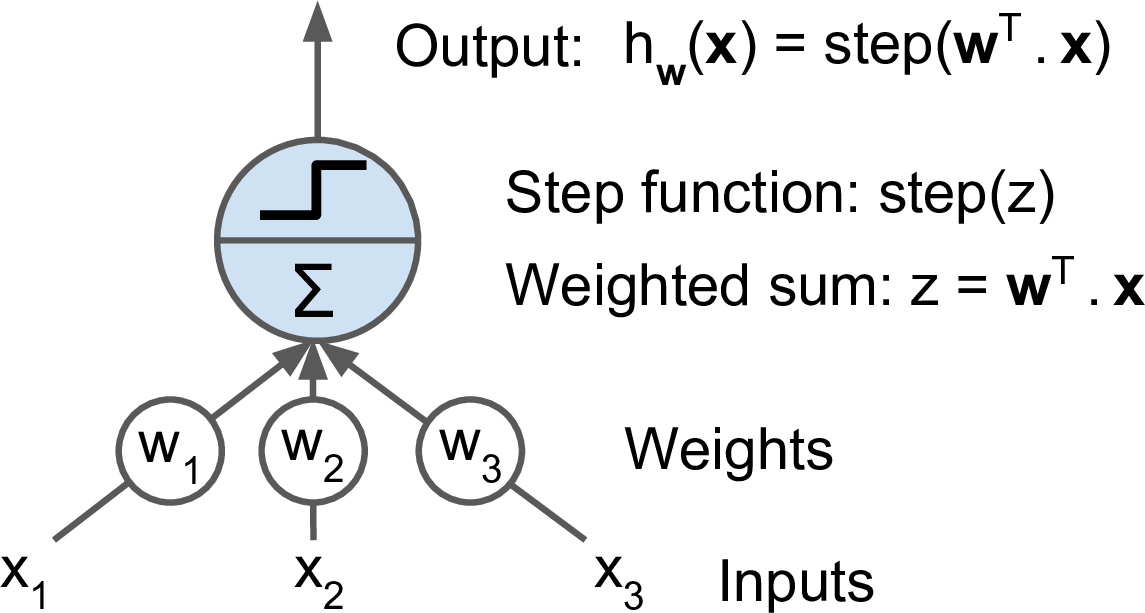
\includegraphics[width=0.50\textwidth]{./images/TLU.png}
\end{figure}

\item
\vspace{-2.0mm}
Traditionally, the activation function was a heavyside step function.
However, in order to perform Gradient Descent on a NN,
a differentiable function was needed instead.\newline
- The default has become the Rectified Linear Unit function: ReLU(z) = max(0,z)\newline
- The logistic function and hyperbolic tangent function are also popular choices.
\end{itemize}
\vspace{-2.0mm}


\textbf{Multilayer Perceptrons (MLPs)} are composed of multiple TLUs as depicted in the diagram.\newline
\textit{The bias neurons are shown, but usually they are implicit.}
\begin{figure}[ht]
\centering
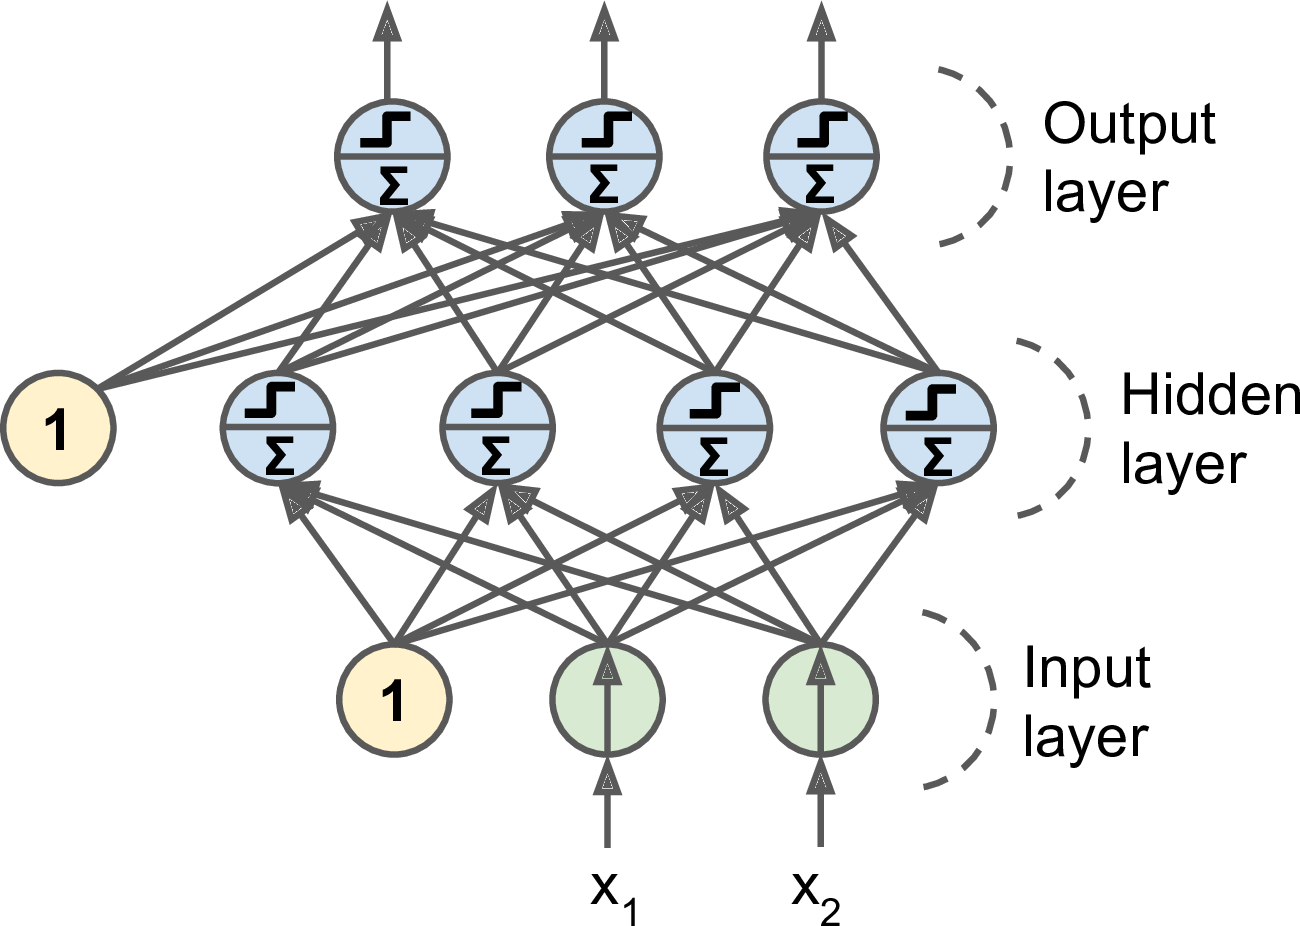
\includegraphics[width=0.50\textwidth]{./images/MLP.png}
\end{figure}

\vspace{-6.0mm}
\begin{itemize}
\item
When there's a deep stack of hidden layers, it is called a \textit{deep neural network (DNN)}.
\item
\vspace{-2.0mm}
Layers close to the input layer are called the \textit{lower layers}\newline
Layers close to the output layer are called the \textit{upper layers}.
\item
\vspace{-2.0mm}
When all the neurons in a layer are connected to every neuron in the previous layer,\newline
the layer is called a \textit{fully connected layer} or a \textit{dense layer}.
\item
\vspace{-2.0mm}
The signal flows only in one direction $=$ \textit{feedforward neural network (FNN)}.
\item
\vspace{-2.0mm}
Without the activation functions, all you would get is a linear model!
\end{itemize}

\newpage
\textbf{Training NNs: Backpropagation}.\newline
In just two passes through the network (one forward, one backward)
the backpropagation algorithm is able to compute the gradient of the network's error
with regard to every single model parameter (i.e. the connection weights),
allowing Gradient Descent to be used to train the NN.

\vspace{-5.0mm}
\begin{itemize}
\item
It handles one mini-batch at a time. The bigger the batch size, the more memory required.

\item
\vspace{-2.0mm}
\textit{The forward pass}.
Each mini-batch is passed through the network.
The output of every neuron is computed and preserved (for every instance in the mini-batch).

\item
\vspace{-2.0mm}
The network's output error is measured.

\item
\vspace{-2.0mm}
\textit{The reverse pass}.
The error gradient across all the connection weights is measured
by propagating the error gradient backward through the network.

\item
\vspace{-2.0mm}
An \textbf{iteration} = one forward-backward pass using one mini-batch.\newline
An \textbf{epoch} = one forward-backward pass of \textit{all} the training set examples.\newline
If you have 2000 training examples, and your batch size is 500...\newline
$\rightarrow$ then it will take 4 iterations to complete 1 epoch.

\item
\vspace{-2.0mm}
It is important to randomly initialize all the hidden layer's connection weights.\newline
This breaks the symmetry and allows backpropagation to train a diverse team of neurons.

\end{itemize}

\textbf{Regression MLPs: Summary}

\begin{tabular}{ |l|l| } 
\hline
Hyperparameter & Typical value \\ 
\hline
Number of input neurons & One per input feature \\ 
Number of hidden layers & Depends on the problem, but typically 1 to 5\\ 
Number of neurons per hidden layer & Depends on the problem, but typically 10 to 100\\ 
Hidden layer activation function & ReLU or SELU\\
Number of output neurons & 1 per prediction dimension\\
Output activation function & In general None (can output any range of values)\\
 & ReLU/softplus (for a positive output contraint)\\
 & Logistic/tanh (for a bounded output contraint)\\
Loss function & Typically MSE (mean squared error)\\
 & Maybe MAE (mean absolute error) when there's lots of outliers\\
\hline
\end{tabular}

\textbf{Classification MLPs: Summary}

\begin{tabular}{ |l|l| } 
\hline
Hyperparameter & Typical value \\ 
\hline
Number of input neurons & One per input feature \\ 
Number of hidden layers & Depends on the problem, but typically 1 to 5\\ 
Number of neurons per hidden layer & Depends on the problem, but typically 10 to 100\\ 
Hidden layer activation function & ReLU or SELU\\
Number of output neurons & 1 (for binary classification)\\
 & 1 per class (for multiclass classification)\\
Output activation function & Logistic (for binary classification)\\
 & Softmax (for multiclass classification)\\
Loss function & Cross entropy\\
\hline
\end{tabular}

\newpage
The architecture of an MLP for multiclass classification:

\begin{figure}[ht]
\centering
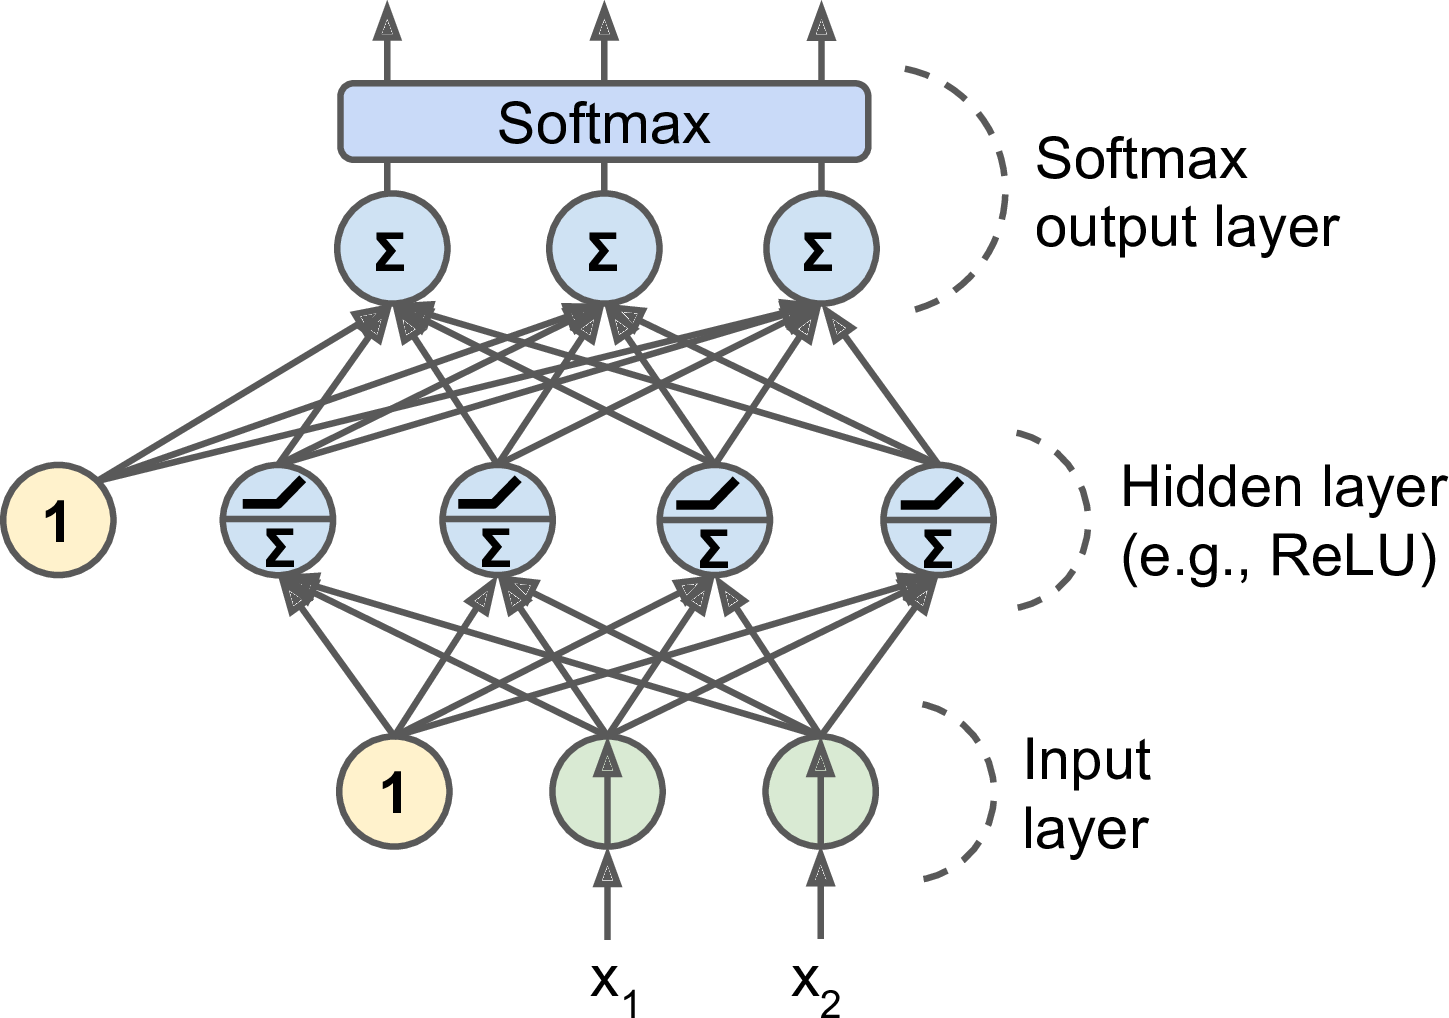
\includegraphics[width=0.50\textwidth]{./images/MLP_classification.png}
\end{figure}

%%%%%%%%%%%%%%%%%%%%%%%%%%%
%%%%%%%%%%%%%%%%%%%%%%%%%%%
%%%%%%%%%%%%%%%%%%%%%%%%%%%
%%%%%%%%%%%%%%%%%%%%%%%%%%%
%%%%%%%%%%%%%%%%%%%%%%%%%%%

\subsection{Implementing MLPs with Keras}

The following code creates a classification MLP with:
\vspace{-5.0mm}
\begin{itemize}
\item
An input layer with 784 neurons, where each instance is a $28*28$ array.
\vspace{-3.0mm}
\item
Two hidden layers (with 300 and 100 neurons, respectively).\newline
Both layers use the ReLU activation function.\newline
All the layers are connected sequentially.
\vspace{-3.0mm}
\item
10 exclusive classification outputs.
\end{itemize}

\vspace{-2.0mm}
\texttt{from tensorflow import keras}\newline
\texttt{model = keras.models.Sequential()}\newline
\texttt{model.add(keras.layers.Flatten(input\char`_shape=[28,28]))}\newline
\texttt{model.add(keras.layers.Dense(300, activation=\textquotesingle relu\textquotesingle))}\newline
\texttt{model.add(keras.layers.Dense(100, activation=\textquotesingle relu\textquotesingle))}\newline
\texttt{model.add(keras.layers.Dense(10, activation=\textquotesingle softmax\textquotesingle))}\newline
\vspace{-2.0mm}

For binary classification, use \texttt{activation=\textquotesingle sigmoid\textquotesingle} (i.e. the logistic function)\newline
For regression, the output layer would be:~\texttt{model.add(keras.layers.Dense(1))}

The following will give a summary of your model:\newline
\textit{Note that `None' in the Output Shape means that the batch size can be anything.}\newline
\texttt{model.summary()}

Each model layer is its own object:\newline
\texttt{input = model.layers[0]}\newline
\texttt{hidden\char`_1 = model.layers[1]}\newline
\texttt{hidden\char`_2 = model.layers[2]}\newline
\texttt{output = model.layers[3]}

Each layer manages its own connection weights between the layers neurons and their inputs:\newline
\texttt{weights, biases = hidden\char`_2.get\char`_weights()}

Notice that the connection weights are randomly initialized (this is required to break symmetry)
and the biases are initialized to zero.\newline
\textit{Sometimes you may want to use a different initialization method (information provided later).}

\newpage
\textbf{Compilation}\newline
After a model is created, you must specify the loss function and the optimizer to use:\newline
\texttt{model.compile(loss=\textquotesingle sparse\char`_categorical\char`_crossentropy\textquotesingle,}\newline
\texttt{.~~~~~~~~~~~~~optimizer=\textquotesingle sgd\textquotesingle,}\newline
\texttt{.~~~~~~~~~~~~~metrics=[\textquotesingle accuracy\textquotesingle]) \# these are optional}

For binary classification: \texttt{loss=\textquotesingle binary\char`_crossentropy\textquotesingle}\newline
For regression: \texttt{loss=\textquotesingle mean\char`_squared\char`_error\textquotesingle}

Note that the optimizer is equivalent to: \texttt{optimizer=keras.optimizers.SGD(lr=0.01)}\newline
\textit{Sometimes you may want to use more efficient optimizers (information provided later).}\newline

\textbf{Training}\newline
\texttt{history = model.fit(X, y, epochs=30, validation\char`_split=0.1)}

- The \texttt{fit()} method returns a History object containing meta-data about the training.\newline
- If not stated, the \texttt{epochs} parameter will default to one (not enough for convergence).\newline
- If not stated, the \texttt{validation\char`_split} parameter will be zero (i.e no cross validation).

Use the History object to plot the learning curves:\newline
\texttt{import pandas as pd}\newline
\texttt{import matplotlib.pyplot as plt}\newline
\texttt{pd.DataFrame(history.history).plot(figsize=(12,8))}\newline
\texttt{plt.grid(True)}\newline
\texttt{plt.gca().set\char`_ylim(0,1)}\newline
\texttt{plt.show()}\newline
\textit{Note that the validation error is computed at the \underline{end} of each epoch,
whilst the training error is computed using a running mean \underline{during} each epoch.}

To continue training, just call the \texttt{fit()} method again. Note the following:\newline
- This will create a new History object (rather than appending).\newline
- You can update the model compilation parameters before the additional training.\newline

\textbf{Evaluation}\newline
Estimate the generalization error using the test set:\newline
\texttt{model.evaluate(X\char`_test, y\char`_test)}

Make predictions as follows:\newline
\texttt{y\char`_proba = model.predict(X\char`_new)}\newline
\texttt{y\char`_pred ~= np.argmax(model.predict(X\char`_new), axis=-1)}\newline

\textbf{Saving and Loading}\newline
The following saves a model's architecture, parameters, and optimizer:\newline
\texttt{model.save(\textquotesingle my\char`_keras\char`_model.h5\textquotesingle)}

The following loads a model:\newline
\texttt{model = keras.models.load\char`_models(\textquotesingle my\char`_keras\char`_model.h5\textquotesingle)}

You can also save your model at regular checkpoints during training...

\newpage
\textbf{Callbacks}\newline
The \texttt{fit()} method accepts a \textit{callbacks} argument
(a list of objects called \underline{during} training).

The following saves your model at regular intervals (default = end of each epoch):\newline
\texttt{save\char`_cb = keras.callbacks.ModelCheckpoint(\textquotesingle my\char`_keras\char`_model.h5\textquotesingle)}\newline
\texttt{history = model.fit(X, y, epochs=10, callbacks=[save\char`_cb])}

Moreover, if you use a validation set during training,
you can ensure your model only saves when the performance on the validation set is the best so far (i.e implicit early stopping):
\texttt{save\char`_cb = keras.callbacks.ModelCheckpoint(\textquotesingle my\char`_keras\char`_model.h5\textquotesingle,\newline
.~~~~~~~~~~~~~~~~~~~~~~~~~~~~~~~~~~~~~~~~~save\char`_best\char`_only=True)}\newline
\texttt{history = model.fit(X, y, epochs=100, validation\char`_split=0.1,\newline
.~~~~~~~~~~~~~~~~~~~callbacks=[save\char`_cb])}

Explicit early stopping can be implemented with the following callback:\newline
\texttt{early\char`_stop\char`_cb = \newline keras.callbacks.EarlyStopping(patience=10, restore\char`_best\char`_weights=True)}

%%%%%%%%%%%%%%%%%%%%%%%%%%%
%%%%%%%%%%%%%%%%%%%%%%%%%%%
%%%%%%%%%%%%%%%%%%%%%%%%%%%
%%%%%%%%%%%%%%%%%%%%%%%%%%%
%%%%%%%%%%%%%%%%%%%%%%%%%%%
\subsection{Fine-Tuning Neural Network Hyperparameters}

The flexibility of NNs is also one of their drawbacks,
there are many hyperparameters to tune:

\vspace{-5.0mm}
\begin{itemize}
\item
\textbf{Learning rate:} very low = $10^{-5}$, keras default = 0.01, very high = 10.\newline
\textit{Always retune this after changing another hyperparameter.}
\item
\textbf{Optimizer:} there are better options out there than mini-batch gradient descent...
\item
\textbf{Batch size:} keras default = 32 (large batch sizes can lead to training instabilities).
\item
\textbf{Hidden layer activation function:} ReLU is a good default in general.
\item
\textbf{Number of hidden layers:} for most problems, you can start with just one or two.
\item
\textbf{Number of neurons:} in general, use the same number for all hidden layers.\newline
\textit{It can sometimes help to make the first hidden layer bigger than the others.}
\item
\textbf{Keras Tuner:} use this library to tune hyperparameters \textit{(keras-team.github.io/keras-tuner/)}
\item
\textbf{Tip:} it's often simpler to pick a model with more layers and neurons than you actually need,
then use early stopping \& other regularization techniques to prevent overfitting.
\end{itemize}
% 
\textbf{Number of hidden layers}\newline
If it has enough neurons, one hidden layer can theoretically model the most complex functions.
% 
However, for complex problems,
deep networks have a much higher \textit{parameter efficiency} than shallow ones:
they can model complex functions using exponentially fewer neurons,
allowing them to reach much better performance with the same amount of training data.
% 
This is because real-world data is often structured in a hierarchial way,
and deep neural networks take advantage of this:\newline
- Lower hidden layers model low-level structures (e.g. line segments).\newline
- Intermediate hidden layers combine these to model intermediate-level structures (e.g. shapes).\newline
- The highest hidden layers combine these to model high-level structures (e.g. faces).\newline
- \textit{Transfer learning} is where you `borrow' the lower layers from a previously trained model.

%%%%%%%%%%%%%%%%%%%%%%%%%%%
%%%%%%%%%%%%%%%%%%%%%%%%%%%
%%%%%%%%%%%%%%%%%%%%%%%%%%%
%%%%%%%%%%%%%%%%%%%%%%%%%%%
%%%%%%%%%%%%%%%%%%%%%%%%%%%
\subsection{Training Deep Neural Networks}

What if you need to tackle a complex problem,
such as detecting hundreds of types of objects in high-resolution images?
% 
You may need to train a much deeper DNN,
perhaps with 10+ layers,
each containing hundreds of neurons.
% 
You might then experience the following problems:

\vspace{-5.0mm}
\begin{itemize}
\item
The \textit{vanishing gradients} or \textit{exploding gradients} problem.
This is when gradients grow ever smaller (or ever larger)
when flowing backward through the DNN during training.
This makes it very hard to train the lower layers.
\vspace{-2.0mm}
\item
Training may be extremely slow.
\vspace{-2.0mm}
\item
A model with millions of parameters risks severly overfitting the training set,
especially if there are not enough training instances or if they are too noisy.
\end{itemize}

\textbf{\underline{The Vanishing Gradients Problem}}\newline
% 
Gradients often get ever smaller as the backpropagation progresses down to the lower layers.
Consequently, the update leaves the lower layers' connection weights virtually unchanged.\newline
This means the training never converges on a good solution.

For the signal to flow properly,
we need the outputs (forward pass) and the gradient (reverse pass) of all the layers to have equal variance.\newline

\textbf{*** Weight Initialization ***}\newline
$fan_{\textrm{in}}$ = the number of inputs into a layer.\newline
$fan_{\textrm{out}}$ = the number of neurons in a layer.\newline
$fan_{\textrm{avg}} = (fan_{\textrm{in}} + fan_{\textrm{out}})/2$.

The connection weights of each layer should be initialized randomly by one of the following:\newline
- Normal distribution with mean 0 and variance $\sigma^2$\newline
- Uniform distribution between $-r$ and $+r$, where $r=\sqrt{3 \sigma^2}$ 

\begin{tabular}{ l|l|l } 

Initialization & Layer Activation function & $\sigma^2$ \\ 
\hline
Glorot & None, tanh, logistic, softmax & $1/fan_{\textrm{avg}}$\\
He & ReLU and variants & $2/fan_{\textrm{in}}$\\
LeCun & SELU & $1/fan_{\textrm{in}}$\\
\end{tabular}

By default, Keras uses Glorit initialization with a uniform distribution when you create a layer.\newline
You can override this like so:\newline
\texttt{keras.layers.Dense(10, activation=\textquotesingle relu\textquotesingle, kernel\char`_initializer=\textquotesingle he\char`_normal\textquotesingle)}
\texttt{keras.layers.Dense(30, activation=\textquotesingle relu\textquotesingle, kernel\char`_initializer=\textquotesingle he\char`_uniform\textquotesingle)}\newline

\textbf{*** Activation Functions ***} \textit{they get better as you go down...}

\textbf{Logistic:} saturates at 0 or 1, with a derivative extremely close to 0. Function has a mean of 0.5.\newline
\textbf{Tanh:} saturates at -1 or 1, with a derivative extremely close to 0. Function has a mean of 0.

\textbf{ReLU:} does not saturate for positive values, and is fast to compute.\newline
During training, some neurons can effectively die (they stop outputting anything other than 0).\newline
This happens when the weighted sum of its inputs are negative for all instances in the training set.
The weights are then no longer updated by Gradient Descent as the gradient is always zero.

\textbf{LeakyReLU} = $\textrm{max}(\alpha z, z)$.
The hyperparameter $\alpha$, typically set to 0.01, defines how much the function `leaks' for $z<0$.
This small slope ensures that leaky ReLUs never die.

\textbf{Exponential Linear Unit (ELU)} = $\alpha(e^z - 1)$ if $z < 0$.
The hyperparameter $\alpha$, typically set to unity, defines the output as $z \rightarrow -\infty$.
This function has a mean value closer to zero and is differentiable at $z=0$.
The use of the exponential function makes it slower to compute.

\textbf{Scaled ELU (SELU):} a scaled variant of ELU ($\alpha = 1.67$ and $scale = 1.05$).\newline
If you build a DNN composed of a sequential stack of dense layers,
and if all hidden layers use the SELU activation function,
then the network will \textit{self-normalize}:
the output of each layer will preserve a mean of 0 and a standard deviation of 1 during training. Conditions:\newline
- The input features must be standardized.\newline
- Every hidden layer's weights must be initialized with LeCun normal initialization. E.g.\newline
\texttt{layers.Dense(10, activation=\textquotesingle selu\textquotesingle, kernel\char`_initializer=\textquotesingle lecun\char`_normal\textquotesingle)}\newline

\textbf{*** Batch Normalization ***}

Although your weight initialization and activation function choice can significantly reduce the danger of vanishing/exploding gradients at the beginning of training,
it doesn't guarantee that they won't come back as the training progresses... Batch Normalization (BN) addresses this.

BN adds an operation in the model just before/after the activation function of each hidden layer.
For each neuron, this operation zero-centres and normalizes the mini-batch instance values.\newline
The results are scaled and shifted using two parameter vectors (two parameters per neuron).\newline
The scaling parameter, $\boldsymbol{\gamma}$, and the shifting parameter, $\boldsymbol{\beta}$, are learnt during training.

\underline{Notes:}\newline
- BN acts like a regularizer, reducing the need for other regularization techniques.\newline
- After training, when making a prediction on a single instance,
an estimated value of the mean and standard deviation for each neuron is used.

\texttt{...}\newline
\texttt{model.add(keras.layers.Flatten(input\char`_shape=[28,28]))}\newline
\texttt{model.add(keras.layers.BatchNormalization())}\newline
\texttt{model.add(keras.layers.Dense(300, activation=\textquotesingle relu\textquotesingle))}\newline
\texttt{model.add(keras.layers.BatchNormalization())}\newline
\texttt{...}\newline

\textbf{*** Gradient Clipping ***}

This technique ensures gradients never exceed some threshold during backpropagation.\newline
It's typically used to mitigate exploding gradients in RNNs.

Each individual gradient component is clipped between -1.0 and 1.0:\newline
\texttt{optimizer = keras.optimizers.SGD(clipvalue=1.0)}

Clip the magnitude of the gradient to 1.0:\newline
\texttt{optimizer = keras.optimizers.SGD(clipnorm=1.0)}

\newpage

\textbf{*** Reusing Pretrained Layers ***}

It is generally not a good idea to train a very large DNN from scratch.
Instead, you should always try to find an existing neural network that accomplishes a similar task,
then reuse the lower layers. This is called \textit{transfer learning}.
It speeds up training and requires less data.\newline

\textbf{\underline{Faster Optimizers}}

Huge training speed boosts can be achieved using a faster optimizer than Gradient Descent:

\textbf{Momentum Optimization:}\newline
$\boldsymbol{m} \leftarrow \beta \boldsymbol{m} - \eta \nabla_{\boldsymbol{\theta}} J (\boldsymbol{\theta})$\newline
$\boldsymbol{\theta} \leftarrow \boldsymbol{\theta} + \boldsymbol{m}$\newline
\texttt{optimizer = keras.optimizers.SGD(lr=0.001, momentum=0.9)}\newline

\textbf{Nesterov Accelerated Gradient (NAG):}\newline
$\boldsymbol{m} \leftarrow \beta \boldsymbol{m} - \eta \nabla_{\boldsymbol{\theta}} J (\boldsymbol{\theta} + \beta \boldsymbol{m})$\newline
$\boldsymbol{\theta} \leftarrow \boldsymbol{\theta} + \boldsymbol{m}$\newline
\texttt{optimizer = keras.optimizers.SGD(lr=0.001, momentum=0.9, nesterov=True)}\newline
Generally, this is faster than regular momentum optimization.\newline

\textbf{RMSProp:}\newline
$\boldsymbol{s} \leftarrow \beta \boldsymbol{s} - (1 - \beta) \nabla_{\boldsymbol{\theta}} J (\boldsymbol{\theta}) \otimes \nabla_{\boldsymbol{\theta}} J (\boldsymbol{\theta})$\newline
$\boldsymbol{\theta} \leftarrow \boldsymbol{\theta} - \eta  \nabla_{\boldsymbol{\theta}} J (\boldsymbol{\theta}) \oslash \sqrt{\boldsymbol{s} + \epsilon} $\newline
\texttt{optimizer = keras.optimizers.RMSprop(lr=0.001, rho=0.9)}\newline
Converges quicker than NAG, but convergence quality might be worse.\newline

\textbf{Adaptive Moment Estimation (Adam):}\newline
$\boldsymbol{m} \leftarrow \beta_1 \boldsymbol{m} - (1 - \beta_1) \nabla_{\boldsymbol{\theta}} J (\boldsymbol{\theta})$\newline
$\boldsymbol{s} \leftarrow \beta_2 \boldsymbol{s} - (1 - \beta_2) \nabla_{\boldsymbol{\theta}} J (\boldsymbol{\theta}) \otimes \nabla_{\boldsymbol{\theta}} J (\boldsymbol{\theta})$\newline
$\widehat{\boldsymbol{m}} \leftarrow \frac{\boldsymbol{m}}{1-\beta_1}$\newline
$\widehat{\boldsymbol{s}} \leftarrow \frac{\boldsymbol{m}}{1-\beta_2}$\newline
$\boldsymbol{\theta} \leftarrow \boldsymbol{\theta} + \eta \, \widehat{\boldsymbol{m}} \oslash \sqrt{\widehat{\boldsymbol{s}} + \epsilon}$\newline
\texttt{optimizer = keras.optimizers.Adam(lr=0.001, beta\char`_1=0.9, beta\char`_2=0.999)}\newline
Often preferred to RMSProp.

Note that since RMSProp and Adam have an adaptive learning rate,
less tuning of the learning rate hyperparameter is required (you can often just use the default $\eta=0.001$).\newline

\textbf{*** Learning Rate Scheduling ***}\newline
If you start with a large learning rate and then reduce it once training stops making fast progress,
you can reach a good solution faster than with the optimal constant learning rate.

\textit{Power scheduling:} $\eta(t) = \eta_0 \, / \, (1 + t/s)$ where $t$ is the iteration number.\newline
\texttt{keras.optimizers.SGD(lr=0.01, decay=1e-4)} where \texttt{decay} is the inverse of $s$.\newline

\newpage

\textbf{\underline{Avoid Overfitting Through Regularization}}

We have already seen \textit{early stopping} and \textit{batch normalization} as forms of regularization.\newline

\underline{$l_1$ and $l_2$ regularization}\newline
This applies an $l_2$ regularization (factor=0.01) to a layer's connection weights.\newline
Note that you should typically to apply the same regularizer to all layers in your NN.\newline
\texttt{keras.layers.Dense(300, activation=\textquotesingle relu\textquotesingle,\newline
.~~~~~~~~~~~~~~~~~~kernel\char`_regularizer=keras.regularizers.l2(0.01)))}\newline

\underline{Dropout}\newline
At every training step, every neuron (including the input neurons, but excluding the outputs)
has a probability $p$ of being ignored.
The hyperparameter $p$ is called the \textit{dropout rate},
and is typically set between 10\% and 50\%.
After training, the neurons don't get dropped anymore (and each input connection weight is multiplied by $1-p$ to align the signal size with training).

Neurons trained with dropout:\newline
- Cannot co-adapt with their neighboring neurons.\newline
- Cannot rely excessively on just a few input neurons.\newline
- Are less sensitive to slight changes in their inputs.

This results in a more robust network that generalizes better.\newline
\textit{You can think of the final NN as an averaged ensemble of lots of smaller NNs.}

\texttt{...}\newline
\texttt{model.add(keras.layers.Flatten(input\char`_shape=[28,28]))}\newline
\texttt{model.add(keras.layers.Dropout(rate=0.2))}\newline
\texttt{model.add(keras.layers.Dense(300, activation=\textquotesingle relu\textquotesingle))}\newline
\texttt{model.add(keras.layers.Dropout(rate=0.2))}\newline
\texttt{...}\newline

Notes:\newline
- In practice, you only need to apply dropout to the top 1-3 layers (excluding the output layer).\newline
- Dropout means the loss evaluation during training can be misleading.\newline
- You need to use \textit{alpha dropout} if you are using the SELU activation function.

\newpage
%%%%%%%%%%%%%%%%%%%%%%%%%%%
%%%%%%%%%%%%%%%%%%%%%%%%%%%
%%%%%%%%%%%%%%%%%%%%%%%%%%%
%%%%%%%%%%%%%%%%%%%%%%%%%%%
%%%%%%%%%%%%%%%%%%%%%%%%%%%
\subsection{TensorFlow}

Around 95\% of use cases do not require anything other than \texttt{tf.keras} and \texttt{tf.data}.\newline
These are TensorFlow's high-level APIs.
But you might need to use the low-level API...\newline

\textbf{\underline{TensorFlow Objects and Operations}}

TensorFlow revolves around \textit{tensors}, which \textit{flow} from operation to operation.\newline
Creating tensors, and using them, is very similar to NumPy:

\texttt{import tensorflow as tf}\newline
\texttt{t = tf.constant([[1., 2., 3.], [4., 5., 6.]])} -- create a tensor.\newline
\texttt{t = tf.constant(a, dtype=tf.float32)} -- create a tensor from a NumPy array.

\texttt{t[:, 1:]} -- an example of indexing.

\texttt{t + 10} -- all sorts of tensor operations are available...\newline
\texttt{tf.square(t)}\newline
\texttt{tf.reduce\char`_mean(t)}\newline
\texttt{t @ tf.transpose(t)}

\texttt{t.dtype} -- note that TensforFlow uses 32-bit floats by default (NumPy uses 64-bit precision).\newline
Also note that TensorFlow does not perform any type conversions automatically.

TensorFlow supports several other data structures:\newline
Variables, sparse tensors, tensor arrays, ragged tensors, string tensors, sets, queues...\newline

\textbf{\underline{Computing Gradients Using Autodiff}}

Use autodiff to efficiently compute gradients. E.g this simple toy function at \texttt{(w1,w2)=(5,3)}.\newline
\texttt{def f(w1, w2):}\newline
\texttt{.~~~return 3*w1**2 + 2*w1*w2}\newline
\texttt{}\newline
\texttt{w1, w2 = tf.Variable(5.), tf.Variable(3.)}\newline
\texttt{with tf.GradientTape() as tape:}\newline
\texttt{.~~~z = f(w1, w2)}\newline
\texttt{gradients = tape.gradient(z, [w1, w2])}

The GradientTape records every operation that involves a Variable data structure.\newline
To save memory, only put the strict minimum inside the tape block.\newline
The tape is automatically erased immediately after you call its \texttt{gradient()} method.\newline

\textbf{\underline{Customizing Keras Models}}

Using TensorFlow's low-level API you can build custom:
% 
\vspace{-5.0mm}
\begin{itemize}
\item
Loss functions.
\vspace{-3.0mm}
\item
Activation functions.
\vspace{-3.0mm}
\item
Initializers.
\vspace{-3.0mm}
\item
Regularizers.
\vspace{-3.0mm}
\item
Layers and Models.
\end{itemize}

\newpage
For better performance,
you should only use vectorized TensorFlow operations.\newline

\textbf{\underline{Custom Loss Functions}}

\texttt{def my\char`_huber(y\char`_true, y\char`_pred):\newline
.~~~error = y\char`_true - y\char`_pred\newline
.~~~is\char`_small\char`_error = tf.abs(error) < 1\newline
.~~~squared\char`_loss = tf.square(error) / 2\newline
.~~~linear\char`_loss = tf.abs(error) - 0.5\newline
.~~~return tf.where(is\char`_small\char`_error, squared\char`_loss, linear\char`_loss)}

def huber_fn(y_true, y_pred):
    error = y_true - y_pred
    is_small_error = tf.abs(error) < 1
    squared_loss = tf.square(error) / 2
    linear_loss  = tf.abs(error) - 0.5
    return tf.where(is_small_error, squared_loss, linear_loss)

\textbf{\underline{Custom Activation Functions, Initializers, and Regularizers}}

def my_softplus(z):
    return tf.math.log(tf.exp(z) + 1.0)

def my_glorot_initializer(shape, dtype=tf.float32):
    stddev = tf.sqrt(2. / (shape[0] + shape[1]))
    return tf.random.normal(shape, stddev=stddev, dtype=dtype)

def my_l1_regularizer(weights):
    return tf.reduce_sum(tf.abs(0.01 * weights))

layer = keras.layers.Dense(1, activation=my_softplus,
                           kernel_initializer=my_glorot_initializer,
                           kernel_regularizer=my_l1_regularizer)

...
model.save("my_model_with_many_custom_parts.h5")

model = keras.models.load_model(
    "my_model_with_many_custom_parts.h5",
    custom_objects={
       "my_l1_regularizer": my_l1_regularizer,
       "my_positive_weights": my_positive_weights,
       "my_glorot_initializer": my_glorot_initializer,
       "my_softplus": my_softplus,
    })
...





Loss functions,
Activation functions,
Regularizers

Custom Loss Functions


If a function has hyperparameters
that need to be saved along with the model... bit more complicated

Custom Layers

1. No weights

2. Create a subclass of the keras.layers.Layer class

Custom Models



\newpage
\section{NAVIGATION}

Note the CMD ALT CNTRL and SHFT on right hand side of keyboard.

General Text:
\begin{easylist}[itemize]
\ListProperties(Style*=$\bullet$ , FinalMark={)}) % FinalMark indicates the end of the list properties and must always be used
& \texttt{SHFT} -- hold to select.
& \texttt{ALT $\leftarrow$ $\rightarrow$} -- jump by word.
& \texttt{CMD $\leftarrow$} -- move cursor to beginning of line.
& \texttt{CMD $\rightarrow$} -- move cursor to end of line.
& \texttt{CMD $\uparrow$} -- move cursor to top of file.
& \texttt{CMD $\downarrow$} -- move cursor to bottom of file.
\end{easylist}

General Apps:
\begin{easylist}[itemize]
\ListProperties(Style*=$\bullet$ , FinalMark={)})
& \texttt{CMD C} -- copy.
& \texttt{CMD X} -- cut.
& \texttt{CMD V} -- paste.
& \texttt{CMD Z} -- undo.
& \texttt{CMD SHFT Z} -- redo.
& \texttt{CMD N} -- new.
& \texttt{CMD O} -- open.
& \texttt{CMD S} -- save.
& \texttt{CMD SHFT S} -- save as.
& \texttt{CMD W} -- close tab.
& \texttt{CMD Q} -- quit.
& \texttt{CMD A} -- select all.
& \texttt{CMD +/-} -- zoom in/out.
& \texttt{CNTRL TAB} -- flick through tabs (use \texttt{SHFT} to reverse).
& \texttt{ALT CMD $\leftarrow$ $\rightarrow$} -- flick through tabs.
& \texttt{CMD <n>} -- select enumerated tab.
\end{easylist}

\newpage
Chrome:
\begin{easylist}[itemize]
\ListProperties(Style*=$\bullet$ , FinalMark={)})
& \texttt{CMD T} -- new tab.
& \texttt{CMD SHFT T} -- re-open closed tab.
& \texttt{CMD L} -- selects location bar.
& \texttt{CMD R} -- reloads page.
\end{easylist}

Finder:
\begin{easylist}[itemize]
\ListProperties(Style*=$\bullet$ , FinalMark={)})
& \texttt{CMD SHFT N} -- create new directory.
\end{easylist}

Mac:
\begin{easylist}[itemize]
\ListProperties(Style*=$\bullet$ , FinalMark={)})
& \texttt{CNTRL CMD Q} -- lock screen.
& \texttt{CNTRL $\leftarrow$ $\rightarrow$} -- flick between pages.
& \texttt{CMD space} -- spotlight search.
& \texttt{CMD tab} -- flick between applications (use \texttt{SHFT} to reverse).
& \texttt{F3} -- desktop info.
& \texttt{F4} -- list of apps.
& \texttt{SHFT CMD 3} -- screenshot.
& \texttt{SHFT CMD 4} -- cropped screenshot.
\end{easylist}

Command Line:
\begin{easylist}[itemize]
\ListProperties(Style*=$\bullet$ , FinalMark={)})
& \texttt{CNTRL U} -- delete from beginning to cursor (up).
& \texttt{CNTRL K} -- delete from cursor to end (kill).
& \texttt{CNTRL W} -- delete previous word (word).
& \texttt{CNTRL Y} -- paste previous delete block.
& \texttt{ALT click} -- move cursor to a specific point.
& \texttt{CNTRL A} -- move cursor to beginning of line.
& \texttt{CNTRL E} -- move cursor to end of line.
& \texttt{CMD $\leftarrow$ $\rightarrow$} -- flicks between terminal sessions.
& \texttt{CMD $\uparrow$ $\downarrow$} -- flicks through past commands \bf{clearly}.
\end{easylist}

Useful Webpages:
\begin{easylist}[itemize]
\ListProperties(Style*=$\bullet$ , FinalMark={)})
& \texttt{https://support.apple.com/en-gb/HT201236} - all the mac shortcuts!
\end{easylist}

\newpage
\section{BASH}

\textit{Everything in UNIX is either a file or a process.
Processes can take additional options.}

Basics:
\begin{easylist}[itemize]
\ListProperties(Style*=$\bullet$ , FinalMark={)}) % FinalMark indicates the end of the list properties and must always be used
& \texttt{cd} -- change directory.
& \texttt{ls} -- list the files/directories.
& \texttt{pwd} -- print working directory.
& \texttt{mkdir} -- make directory.
& \texttt{touch} -- create file.
& \texttt{rm, rmdir} -- remove.
& \texttt{cp} -- copy
& \texttt{mv} -- move (rename)
& \texttt{echo} -- print to command line.
& \texttt{wc} -- word count.
\end{easylist}

Other:
\begin{easylist}[itemize]
\ListProperties(Style*=$\bullet$ , FinalMark={)}) % FinalMark indicates the end of the list properties and must always be used
& \texttt{file <file>} -- tells you what type of file it is.
& \texttt{tar} -- (un)compress files and directories. 
& \texttt{du -sh} -- check the disk usage.
& \texttt{df [path]} -- reports on amount of available disk space.
& \texttt{ps [ux[ww]]} -- gives you info abouts your processes. 
& \texttt{top} -- gives you info abouts the systems processes.
& \texttt{who} -- see who is on the system with you.
& \texttt{chmod X$\pm$Y} -- change permissions.\newline\textbf{X} = \texttt{u}:user, \texttt{g}:group, \texttt{o}:other, \texttt{a}:all. \textbf{Y} = \texttt{r}:read, \texttt{w}:write, \texttt{x}:execute.
& \texttt{<command> --help, man <command>} -- how to use a command.
& \texttt{say <quote>} -- voice output from the terminal.
& \texttt{open -a [application] filename} -- open a file.
% & \texttt{date} -- displays the date and time.
& \texttt{echo one two three | xargs mkdir} -- xargs allows tools to accept standard input as arguments.
\end{easylist}

Navigation:
\begin{easylist}[itemize]
\ListProperties(Style*=$\bullet$ , FinalMark={)}) % FinalMark indicates the end of the list properties and must always be used
& \texttt{/} -- root directory.
& \texttt{./} -- current directory, alias for \texttt{\$PWD}.
& \texttt{../} -- parent directory.
& $\sim$ -- home directory, alias for \texttt{\$HOME}.
& \texttt{-} -- previous directory, alias for \texttt{\$OLDPWD}.
& \texttt{dirs} -- directory stack. By default the first value is \texttt{\$PWD}. \verb!-c! cleans stack. \verb!-v! shows enumerated version; cd into them using \verb!cd! $\sim$\verb!n!.
& \texttt{pushd .} -- add current directory to stack. 
& \texttt{*} -- wildcards for file and directory names.
& \texttt{?} -- single character wildcards.
& \texttt{Tab} -- auto complete until an ambiguity arises.
& \texttt{Tab Tab} -- displays the ambiguities.
\end{easylist}

Text:
\begin{easylist}[itemize]
\ListProperties(Style*=$\bullet$ , FinalMark={)}) % FinalMark indicates the end of the list properties and must always be used
& \texttt{cat, head, tail} -- display text file (all, top, bottom).
& \texttt{more} -- scroll through text file (space bar for next page).
& \texttt{sort <stream/file>} -- sort text.
& \texttt{diff} -- differences between files.
& \texttt{command > file} -- redirect standard output to a file (use \verb!>&! to include errors).
& \texttt{command >> file} -- append standard output to a file.
& \texttt{command1 | command2} -- pipe output of command-1 to input of command-2.
\end{easylist}

History and Kill:
\begin{easylist}[itemize]
\ListProperties(Style*=$\bullet$ , FinalMark={)}) % FinalMark indicates the end of the list properties and must always be used
& $\uparrow$ and $\downarrow$ -- scroll command history.
& \texttt{history} -- show command history (use \texttt{grep} to filter).
& \texttt{CNTRL R} -- navigate bash history (press repeatedly to search further back).
& \texttt{clear} -- clears the screen.
& \texttt{CNTRL C} -- kill a foreground process in the foreground.
\newpage
& \texttt{CNTRL Z} -- put a foreground process in the background. Use \texttt{\&} at the end of a command to do this automatically.
& \texttt{bg} -- look at background processes, provides a job number.
& \texttt{fg \% <jobNumber>} -- put background process in foreground.
& \texttt{kill \% <jobNumber>} -- kill background process.
\end{easylist}

Very Useful, Can Never Remember:
\begin{easylist}[itemize]
\ListProperties(Style*=$\bullet$ , FinalMark={)}) % FinalMark indicates the end of the list properties and must always be used
& \texttt{sed} -- \textbf{s}tream \textbf{ed}itor. 
& \texttt{sed \textquotesingle s/<old>/<new>/g\textquotesingle~<stream/file>} -- sed for substitution.
\newline Use \verb!-i! for in-file replacement. Note you can use different delimiters.
& \texttt{find <directory> -name <file name>} -- find the path to a file.\newline Searches recursively by default. Other options exist e.g. file size.
& \texttt{grep <expression> <stream/file>} -- search text file for an expression.
\newline Option \verb!-i! ignores case; \verb!-r! searches recursively.
\end{easylist}

Secure Shell:
\begin{easylist}[itemize]
\ListProperties(Style*=$\bullet$ , FinalMark={)}) % FinalMark indicates the end of the list properties and must always be used
& \texttt{scp <local path> <user>@<hostname>:<destination path>} \newline-- secure copy.
& \texttt{ssh -XY <user>@<hostname>} -- secure shell, to log in to a remote server.
& \texttt{sshfs <user>@<hostname>:/path/to/base/ <locMountDir> -o volname=NAME} -- secure shell file system.
& \texttt{display <image file>} -- view things in ssh.
& \texttt{exit} -- exit ssh session.
\end{easylist}

Screen:
\begin{easylist}[itemize]
\ListProperties(Style*=$\bullet$ , FinalMark={)}) % FinalMark indicates the end of the list properties and must always be used
& \texttt{screen} -- start screen session (environments are not transferred over). 
& \texttt{Ctrl A} then \texttt{D} -- detach screen session. 
& \texttt{exit} -- kill screen session. 
& \texttt{screen -r <sessionID>} -- re-attach screen session. 
& \texttt{screen -ls} -- list screen sessions. 
& \texttt{screen -X -S <sessionID> kill} -- kill screen session without attaching it. 
\end{easylist}

\newpage
Environment Variables And Loops:
\begin{easylist}[itemize]
\ListProperties(Style*=$\bullet$ , FinalMark={)}) % FinalMark indicates the end of the list properties and must always be used
& \texttt{env} -- print environmental variables. \texttt{PATH} is a colon seperated list of dirs that your shell searches for an executable.
& \texttt{export PATH="/path/to/bin:\$PATH"} -- example of setting an environmental variable.
& \texttt{myvar=123abc} -- example of declaring a variable (string only).
& \texttt{echo \$myvar} -- example of using variable.
& \texttt{for myvar in *.pdf; do ls \$myvar; echo; done} \newline-- specific example of for loop.
& \texttt{while true; do <command1>; <command2>; etc; done} \newline-- run a command periodically.
& \texttt{alias <shortcut>="<regularExpression>"} -- alias commands.
& \texttt{source <shell file>} -- evaluates the file.
& \texttt{.bashrc} OR \texttt{.bash\char`_profile} -- for permanent aliases and setting of variables.
\end{easylist}

Useful Webpages:
\begin{easylist}[itemize]
\ListProperties(Style*=$\bullet$ , FinalMark={)}) % FinalMark indicates the end of the list properties and must always be used
& \texttt{https://ss64.com/bash/} -- all the commands!
\end{easylist}

\newpage
\section{EMACS}

\vspace{\baselineskip}

Edit text files quickly without using a full blown text editor.

\begin{easylist}[itemize]
\ListProperties(Style*=$\bullet$ , FinalMark={)})
& \texttt{emacs [-nw] <file>} -- open/create a file to edit (no window system).
& \texttt{CMD C and CMD V} -- normal copy and paste commands work.
& \texttt{CNTRL X then CNTRL S} -- save file.
& \texttt{CNTRL X then CNTRL C} -- exit file (if changes not saved you'll have to answer questions).
& \texttt{CNTRL X then U} -- undo.
& \texttt{CNTRL space} -- set marker.
& \texttt{CNTRL W} -- kill marker.
& \texttt{CNTRL K} -- kill from cursor to end of line.
& \texttt{CNTRL Y} -- undo kill.
& \texttt{CNTRL S} -- search forward.
& \texttt{CNTRL R} -- search backward.
\end{easylist}

\vspace{\baselineskip}
\vspace{\baselineskip}
\vspace{\baselineskip}
\vspace{\baselineskip}

How to get the hell of Vi or Vim - without saving.
\begin{easylist}[itemize]
\ListProperties(Style*=$\bullet$ , FinalMark={)})
& \texttt{ESC} -- to enter `normal' mode.
& \texttt{type :q!} -- quit without saving command.
& \texttt{ENTER} -- execute.
\end{easylist}

\vspace{\baselineskip}
\vspace{\baselineskip}

How to get the hell of Nano.
\begin{easylist}[itemize]
\ListProperties(Style*=$\bullet$ , FinalMark={)})
& \texttt{CNTRL X} -- to exit nano.
\end{easylist}

\newpage
\section{SUBLIME}

Colour schemes can be selected via: Sublime Text $\rightarrow$ Preferences $\rightarrow$ Color Scheme...
\newline
Preferences can be set in: Sublime Text $\rightarrow$ Preferences $\rightarrow$ Settings (\texttt{CMD ,} )
\begin{easylist}[itemize]
\ListProperties(Style*=$\bullet$ , FinalMark={)}) % FinalMark indicates the end of the list properties and must always be used
& \texttt{"auto{\char`_}find{\char`_}in{\char`_}selection": true}
& \texttt{"font{\char`_}size": 12}
& \texttt{"word{\char`_}wrap": false}
& \texttt{"translate{\char`_}tabs{\char`_}to{\char`_}spaces": true}
\end{easylist}

Short-Cut basics:
\begin{easylist}[itemize]
\ListProperties(Style*=$\bullet$ , FinalMark={)})
& \texttt{CMD Z} -- undo.
& \texttt{CMD Y} -- redo.
& \texttt{CMD C} -- copy.
& \texttt{CMD X} -- cut.
& \texttt{CMD V} -- paste.
& \texttt{CMD SHIFT V} -- paste with indent.
\end{easylist}

Short-Cut Lines:
\begin{easylist}[itemize]
\ListProperties(Style*=$\bullet$ , FinalMark={)})
& \texttt{CNTRL CMD $\uparrow$ $\downarrow$} -- swap line up or down.
& \texttt{CMD SHFT D} -- duplicate line (does not use clipboard).
& \texttt{CNTRL SHFT K} -- delete line.
& \texttt{CNTRL K} -- delete line to end.
& \texttt{CMD delete} -- delete line to beginning.
& \texttt{CMD J} -- join lines.
\end{easylist}

Short-Cut Text:
\begin{easylist}[itemize]
\ListProperties(Style*=$\bullet$ , FinalMark={)})
& \texttt{CMD ]} -- indent.
& \texttt{CMD [} -- un-indent.
& \texttt{CMD /} -- toggle comments.
& \texttt{CMD ENTER} -- insert line afterwards (don't need to be on end of current line).
& \texttt{CMD SHFT ENTER} -- insert line before.
& \texttt{CNTRL T} -- swaps two characters around (transpose).
& \texttt{CMD K} then \texttt{U} -- convert to upper case.
& \texttt{CMD K} then \texttt{L} -- convert to lower case.
\end{easylist}

Short-Cut Selection. \textit{Remember mouse middle button selection:}
\begin{easylist}[itemize]
\ListProperties(Style*=$\bullet$ , FinalMark={)})
& \texttt{CMD A} -- select all.
& \texttt{CMD D} -- select word.
& \texttt{CMD L} -- select (full) lines.
& \texttt{CNTRL SHFT M} -- select within brackets.
& \texttt{CMD SHFT J} -- select within indentation.
& \texttt{CMD SHFT space} -- select within scope.
\end{easylist}

Find and Replace:
\begin{easylist}[itemize]
\ListProperties(Style*=$\bullet$ , FinalMark={)})
& \texttt{CMD F} -- set up find (press \texttt{escape} to leave). Note the special options available.\newline \textit{Select the area you wish to use.}
& \texttt{ENTER} -- find next (hold \texttt{SHFT} to reverse this).
& \texttt{ALT ENTER} -- to replace.
\end{easylist}

Other:
\begin{easylist}[itemize]
\ListProperties(Style*=$\bullet$ , FinalMark={)})
& \texttt{F6} -- spell check.
& \texttt{CNTRL F6} -- next misspelled word.
\end{easylist}

\newpage
\section{GITHUB}

Git is a version control system.
GitHub is the online store.

\vspace{\baselineskip}
GitHub -- i.e. online:
\begin{easylist}[itemize]
\ListProperties(Style*=$\bullet$ , FinalMark={)}) % FinalMark indicates the end of the list properties and must always be used
&
To setup a new repository online you must first create an \textbf{empty} repo on GitHub.
In your local repo, you can then set this new GitHub repo as the remote.
% And then you're off.
&
If you want to collaborate on an existing repo, you should fork this repo to your account.
To get it locally you should then clone the GitHub version of the repo.
&
If you want to merge your code with a collaborator on GitHub, use the `New Pull Request' button.
\end{easylist}

Git Setup:
\begin{easylist}[itemize]
\ListProperties(Style*=$\bullet$ , FinalMark={)}) % FinalMark indicates the end of the list properties and must always be used
& \texttt{git init [projectDir]} -- setup git. You will be on a branch called `master'.
& \texttt{git clone git@github.com:joseph-taylor/LjLabBook.git <localRepoName>} -- clone a repo to local from GitHub.
This will automatically set a remote called `origin'.
& \texttt{.gitignore} -- text file telling git what files to ignore.
& \texttt{git config --global core.editor "emacs -nw"} -- set emacs as default git text editor.
\end{easylist}

Git Basics:
\begin{easylist}[itemize]
\ListProperties(Style*=$\bullet$ , FinalMark={)}) % FinalMark indicates the end of the list properties and must always be used
& \texttt{git status} -- prints the status of your branch.
& \texttt{git add <files>} -- stages changes to files.
& \texttt{git reset HEAD <files>} -- unstage files.
& \texttt{git rm <files>} -- remove files and have git stage the changes.
& \texttt{git mv <files> <location>} -- move files and have git stage the changes.
& \texttt{git commit [-m "message"]} -- commit the changes.
\end{easylist}

Git Commit Labels:
\begin{easylist}[itemize]
\ListProperties(Style*=$\bullet$ , FinalMark={)}) % FinalMark indicates the end of the list properties and must always be used
& Each commit is labelled by a commit hash. Use \texttt{git} \texttt{log} to find them.
& \texttt{HEAD} -- a special label referring to your current commit on your current branch.
& \texttt{commitLabel\^{}} -- refers to a NEW label, one commit before the label provided.
& \texttt{commitLabel\^{}\^{}} -- refers to a NEW label, two commits before the label provided.
& \texttt{commitLabel$\sim$N} -- refers to a NEW label, N commits before the label provided.
\end{easylist}

\newpage
Git Useful:
\begin{easylist}[itemize]
\ListProperties(Style*=$\bullet$ , FinalMark={)}) % FinalMark indicates the end of the list properties and must always be used
& \texttt{git diff <file>} -- diff between current file and version from last commit.
& \texttt{git diff <commitLabel> <file>} -- diff between current file and version from the stated commit.
& \texttt{git diff <commitLabelOne> <commitLabelTwo> <file>} -- diff between file for two different commits.
& \texttt{git log} -- log of git commit messages and hashes.
& \texttt{git help <command>} -- git help pages.
\end{easylist}

Git Branching
(note that you get conflicts when changes are made to the same files):
\begin{easylist}[itemize]
\ListProperties(Style*=$\bullet$ , FinalMark={)}) % FinalMark indicates the end of the list properties and must always be used
& \texttt{git checkout -b <newBranchName>} -- create new branch and change to it
\newline (modifications in the repo \textbf{are} carried over).
& \texttt{git checkout <oldBranchName>} -- change to an existing branch.
& \texttt{git merge <branchNameToMerge> [-m "message"]} -- merge changes from stated branch into current branch.
& \texttt{git branch -d <branchNameToDelete>} -- delete branch (can only do this if the changes are merged).
\end{easylist}

Git Stashing
(if you want to change branch, but don't want to commit current work first):
\begin{easylist}[itemize]
\ListProperties(Style*=$\bullet$ , FinalMark={)})
& \texttt{git stash} -- saves your changes and goes back to the HEAD commit.
& \texttt{git stash list} -- look at your stored stashes.
& \texttt{git stash apply [stash@\{N\}]} -- apply a stash. If you have more than one stash you should name it.
& \texttt{git stash clear} -- remove all stashes.
& \texttt{git stash drop <stash@\{N\}>} -- remove a specific stash.
\end{easylist}

Reversing Changes in Git:
\begin{easylist}[itemize]
\ListProperties(Style*=$\bullet$ , FinalMark={)}) % FinalMark indicates the end of the list properties and must always be used
& \texttt{git checkout -- <file>} -- undo uncommited changes to a file (the \texttt{--} avoids conflict with branch names).
& \texttt{git checkout <commitLabel>} --  detached HEAD state: can view state of old commit but you are not on a branch. Branch off if you want to work from here.
& \texttt{git revert <commitLabel>} -- reverses \textbf{the changes of} the stated commit. This change happens in the form of a new commit. Just exit the emacs situation.
& \texttt{git reset <commitLabel>} -- moves a branch back in time to an older commit. The commits that were on top of it no longer exist. Not good when collaborating.
\end{easylist}

\newpage
Git to GitHub:
\begin{easylist}[itemize]
\ListProperties(Style*=$\bullet$ , FinalMark={)}) % FinalMark indicates the end of the list properties and must always be used
& \texttt{git remote [-v]} -- print the GitHub remotes for the repo.
& \texttt{git remote add <remoteName> git@github.com:joseph-taylor/LjLabBook.git} -- create a new remote.
& \texttt{git push <remoteName> <branchName>} -- push commits on the local branch to the remote branch (you don't have to be on that branch).
& \texttt{git pull <remoteName> <branchName>} -- pull commits on remote branch to the local branch (you don't have to be on that branch).
\end{easylist}

\vspace{\baselineskip}
\vspace{\baselineskip}
Useful Webpages
\begin{easylist}[itemize]
\ListProperties(Style*=$\bullet$ , FinalMark={)}) % FinalMark indicates the end of the list properties and must always be used
& \texttt{https://learngitbranching.js.org/} - practise git branching conceputally.
& \texttt{https://help.github.com/articles/connecting-to-github-with-ssh/} - connecting to GitHub with SSH.
\end{easylist}

\newpage
\section{PYTHON}

\vspace{\baselineskip}
\textbf{GENERAL PYTHON}\newline
I learnt python at
\texttt{http://chryswoods.com/main/courses.html}

\vspace{\baselineskip}
\textbf{ANACONDA}\newline
Anaconda has access to over 720 packages that can easily be installed with Anaconda's conda, a package, dependency, and environment manager.\newline
\texttt{https://www.anaconda.com/download/\#macos}

\vspace{\baselineskip}
\textbf{JUPITER NOTEBOOKS}\newline
\texttt{https://www.datacamp.com/community/tutorials/tutorial-jupyter-notebook} \newline
Jupiter notebooks run on your browser.
They are like ipython sessions that can be saved.
You can also edit previous lines.
Also lots of other features to explore.\newline
\begin{easylist}[itemize]
\ListProperties(Style*=$\bullet$ , FinalMark={)})
& \texttt{jupyter notebook} -- to set it all up.\newline Then start a new notebook or select an old .ipynb file.
& \texttt{SHFT ENTER} -- run cell and select next.
\end{easylist}

\vspace{\baselineskip}
\textbf{PYTORCH}\newline
\texttt{https://pytorch.org/tutorials/}

\vspace{\baselineskip}
\vspace{\baselineskip}
\vspace{\baselineskip}
\vspace{\baselineskip}


numPy
scyPy
matplotlib
pandas + dataframes
FREE BOOK AND NOTEBOOKS
https://github.com/jakevdp/PythonDataScienceHandbook
FREE COURSE TYPE THINGY
https://www.lynda.com/Numpy-tutorials/Introduction-Data-Analysis-Python/419162-2.html


tensorFlow:::keras
http://playground.tensorflow.org/

\newpage
\section{NUMPY}

\vspace{\baselineskip}
\textit{Note that lots of linear algebra methods are available...}
\newline

Array Creation:
\begin{easylist}[itemize]
\ListProperties(Style*=$\bullet$ , FinalMark={)})
& \texttt{a = np.array([1, 2, 3, 4])} ~-- creation using a python array.
& \texttt{A = np.array([[1, 2, 3, 4], [5, 6, 7, 8]])} ~-- \textit{another example}.
\newline
& \texttt{b = np.zeros(5)} ~-- creates a 1D array of zeros.
& \texttt{B = np.zeros((10, 5))} ~-- creates a multi-dimensional array of zeros.
\newline
& \texttt{c = np.ones(3)} ~-- creates a 1D array of ones.
& \texttt{C = np.ones((12, 12, 3))} ~-- creates a multi-dimensional array of ones.
\newline
& \texttt{d = np.random.randn(8)} ~-- creation using random numbers.
& \texttt{D = np.random.normal(100, 3, (8,4))} ~-- \textit{another example}.
\newline
& \texttt{v = np.arange(10, 30, 0.5)} ~-- from 10 to 30 (not included) in steps of 0.5.
& \texttt{v = np.linspace(0, 20, 5000)} ~-- from 0 to 20 (it \textbf{is} included) in 5000 steps.
\end{easylist}

\vspace{\baselineskip}
Basic Operations (they are performed \textit{elementwise}):
\begin{easylist}[itemize]
\ListProperties(Style*=$\bullet$ , FinalMark={)})
& \texttt{C = A**2} ~-- square every element.
& \texttt{C = A + B} ~-- add every equivalent element.
& \texttt{C = A * B} ~-- multiply every equivalent element.
& \texttt{C = 10 * np.sin(A)} ~-- apply a function to every element.
& \texttt{C = (A < 10)} ~-- apply logic to every element.
\newline
& \texttt{A @ B} ~-- matrix dot product.
& \texttt{A.max()} ~-- built-in array functionality.
& \texttt{A.min()} ~-- \textit{another example}.
& \texttt{A.sum()} ~-- \textit{another example}.
\end{easylist}

Indexing, Slicing, and Iterating:
\newline
\newline
\textbf{Note that the first elements are indexed by zero.}
\begin{easylist}[itemize]
\ListProperties(Style*=$\bullet$ , FinalMark={)})
& \texttt{M[i, j, k, ...]} ~-- get the \textit{i$^{\textrm{th}}$} row, ~\textit{j$^{\textrm{th}}$} column, ~\textit{k$^{\textrm{th}}$} `depth', etc...
\newline
& \texttt{v[-n]} ~-- get the \textit{n$^{\textrm{th}}$} last element in the array.
& \texttt{v[3:6]} ~-- get row elements indexed from 3 up to (but not including) 6.
& \texttt{v[:6]} ~-- get row elements indexed from \textbf{the beginning} up to (but not including) 6.
& \texttt{v[3:]} ~-- get row elements indexed from 3 up to \textbf{the end}.
& \texttt{v[27:62:4]} ~-- get elements indexed from 27 up to (but not including) 62 in steps of 4.
& \texttt{v[62:27:-1]} ~-- get elements indexed from 62 down to (but not including) 27.
& \texttt{v[~:~:-1]} ~-- \textit{another example}: reverses a 1D array.
\newline
& \texttt{M[:, 2]} ~-- returns an array of all the matrix row elements for the column with index=2.
& \texttt{M[5, :]} ~-- returns an array of all the matrix column elements for the row with index=5.
& \texttt{M[5]} ~-- when not enough indices provided, those missing are considered complete slices.
\newline
& \texttt{for i in v: print i} ~-- iterate over elements in 1D array.
& \texttt{for row in M: print row} ~-- iterate over first axis in multi-dimensional arrays.
\end{easylist}

\vspace{\baselineskip}
Shape Manipulations:
\begin{easylist}[itemize]
\ListProperties(Style*=$\bullet$ , FinalMark={)})
& \texttt{M.shape} ~-- returns the matrix shape (rows, columns, `depths', etc).
& \texttt{M.ravel()} ~-- puts the object into a 1D array format.
& \texttt{M.reshape(4, 3, 2)} ~-- puts the object into the given matrix shape.
& \texttt{M.reshape(4, -1, 2)} ~-- one of the dimensions does not need specifying.
\newline
& \texttt{C = np.vstack([A, B])} ~-- vertically concatenate objects.
& \texttt{C = np.hstack([A, B])} ~-- horizontally concatenate objects.
\end{easylist}

\newpage
\begin{figure}[ht]
\centering
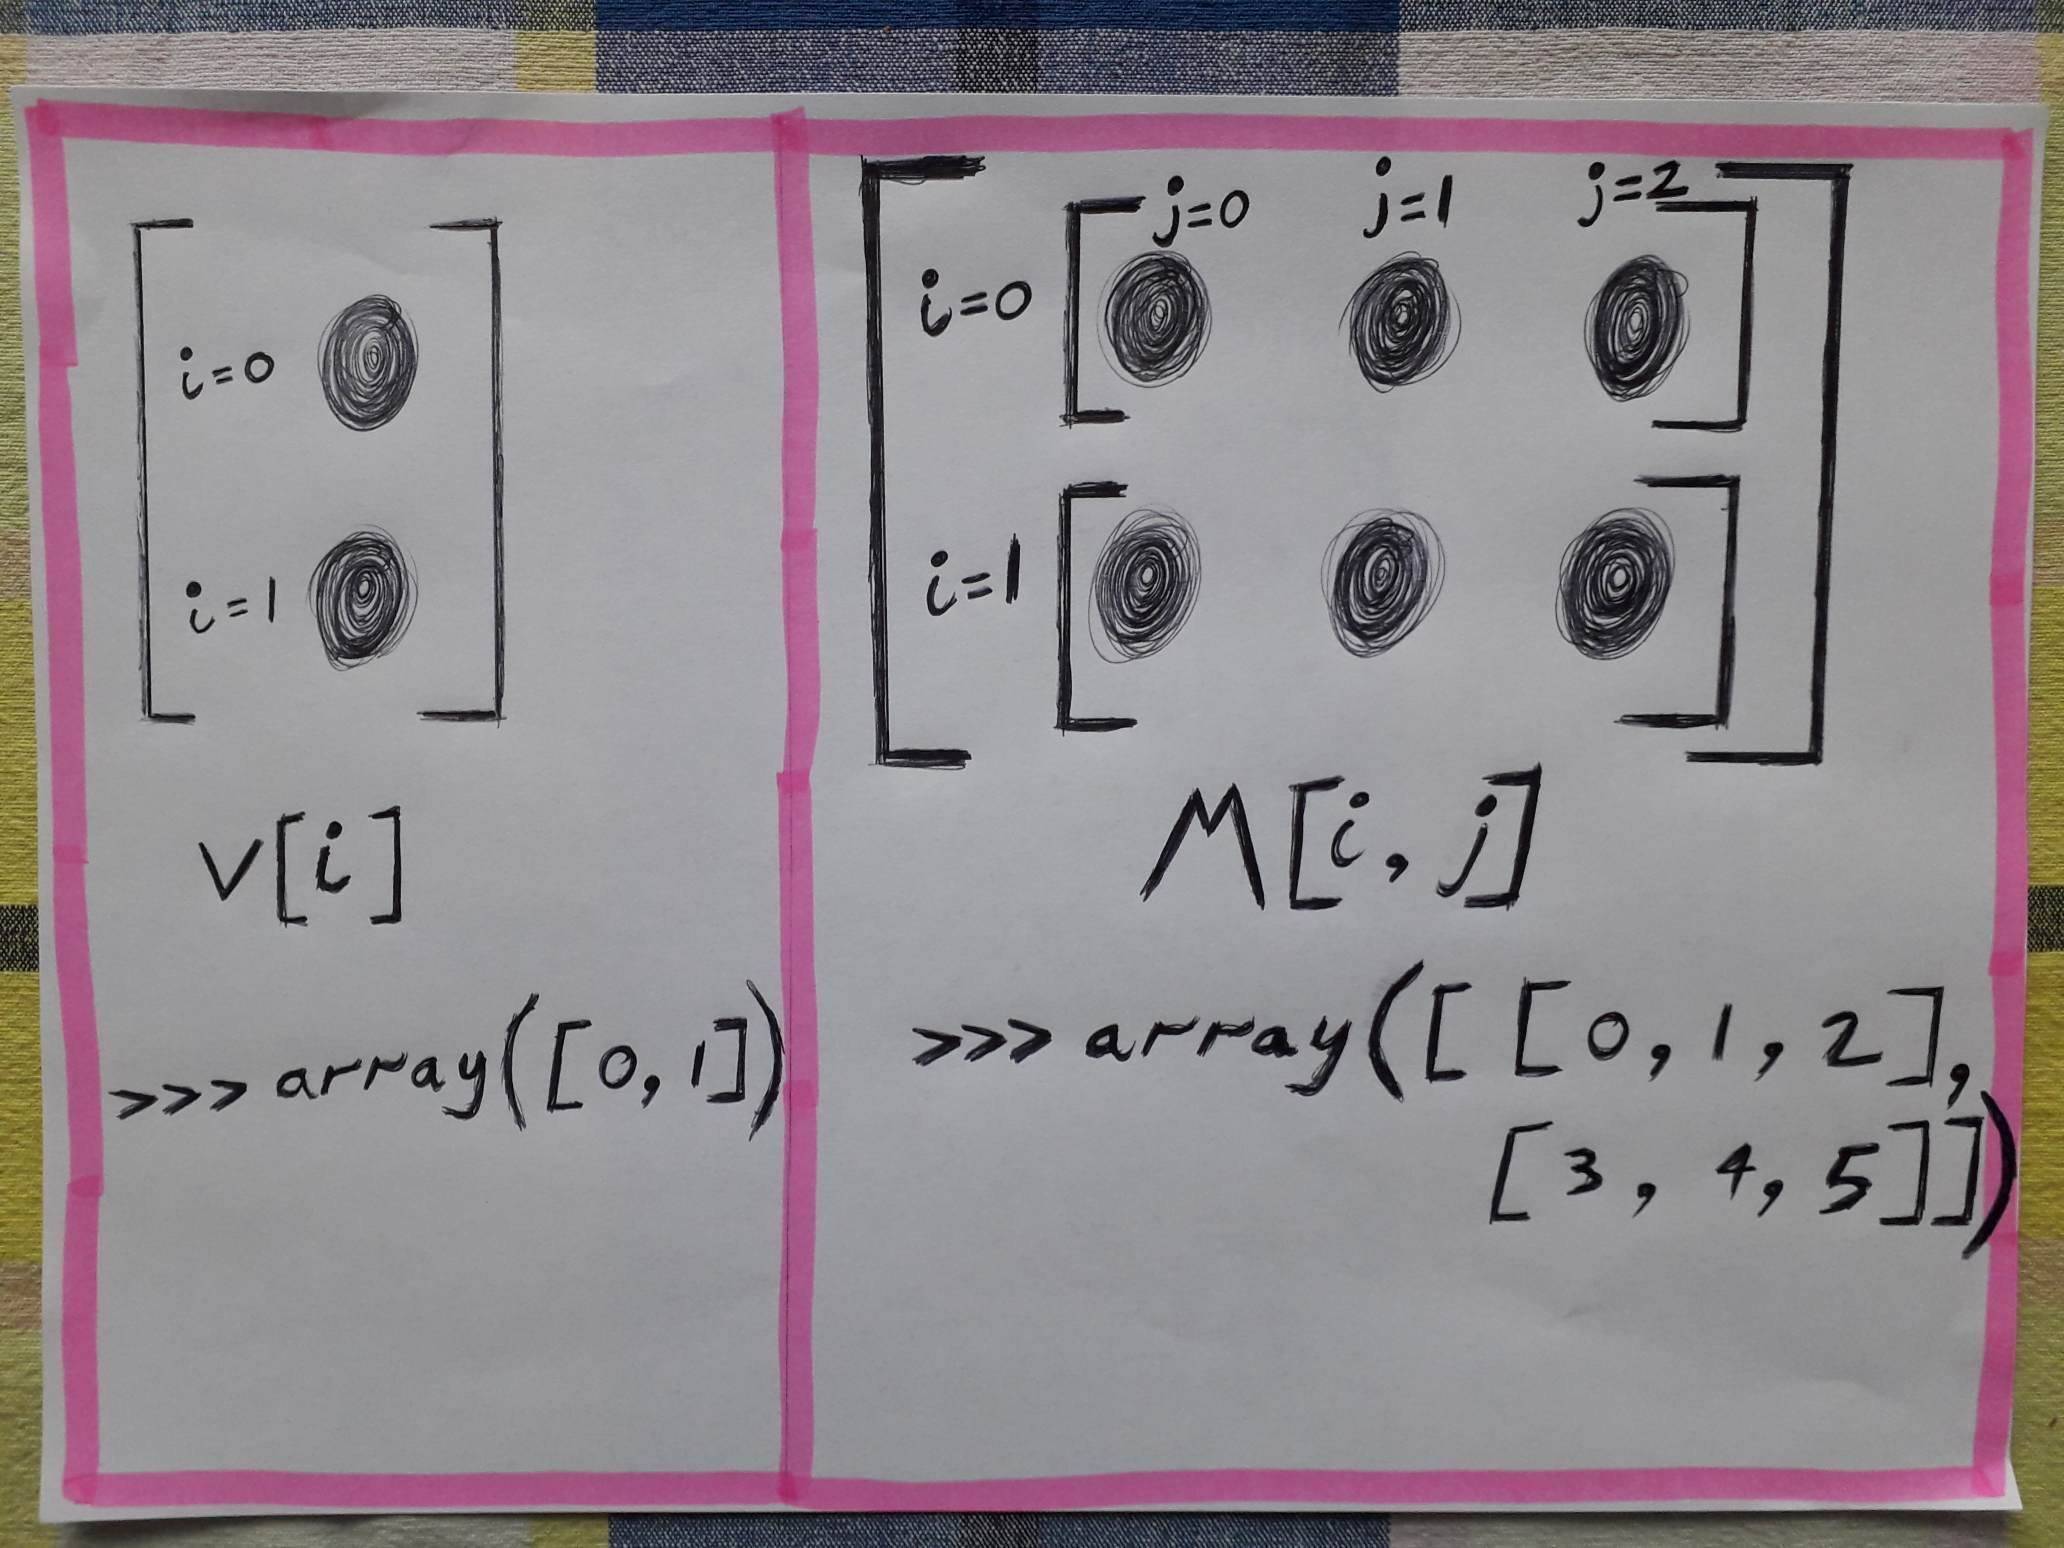
\includegraphics[width=1.00\textwidth]{./images/1d_2d_array.jpg}
\caption{
Visualization of 1D and 2D arrays, respectively.
}
\label{fig:1d_2d_array}
\end{figure}

\newpage
\begin{figure}[ht]
\centering
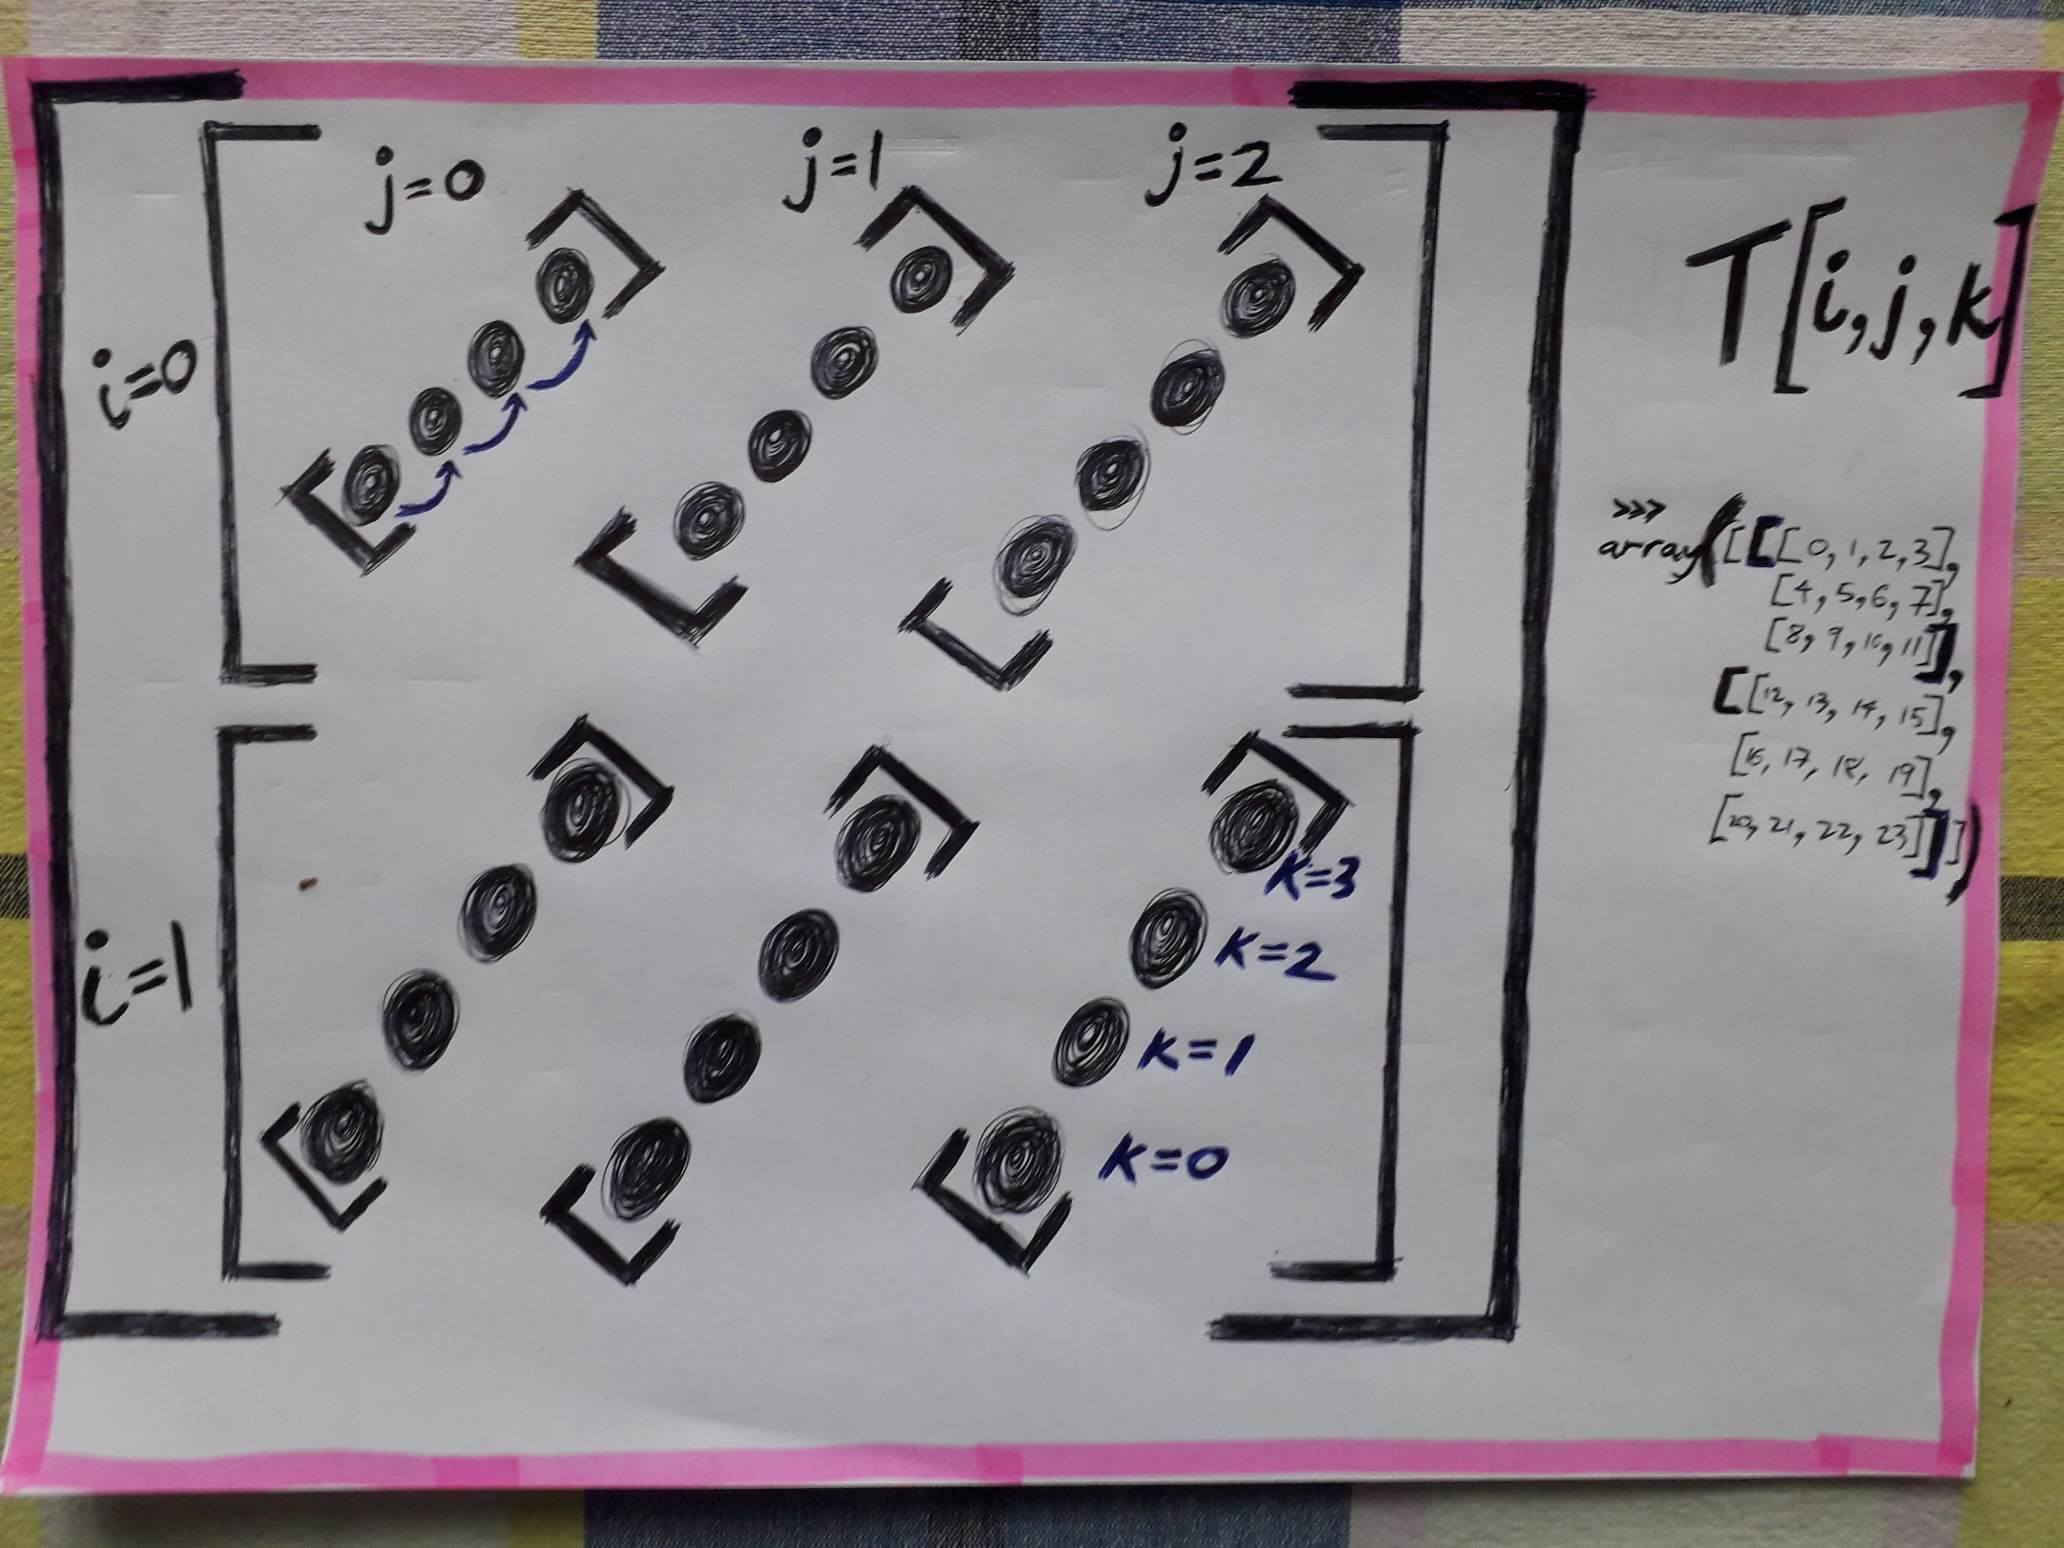
\includegraphics[width=1.00\textwidth]{./images/3d_array.jpg}
\caption{
Visualization of 3D arrays.
}
\label{fig:3d_array}
\end{figure}

\vspace{\baselineskip}
\vspace{\baselineskip}
\vspace{\baselineskip}
\vspace{\baselineskip}

\begin{figure}[ht]
\centering
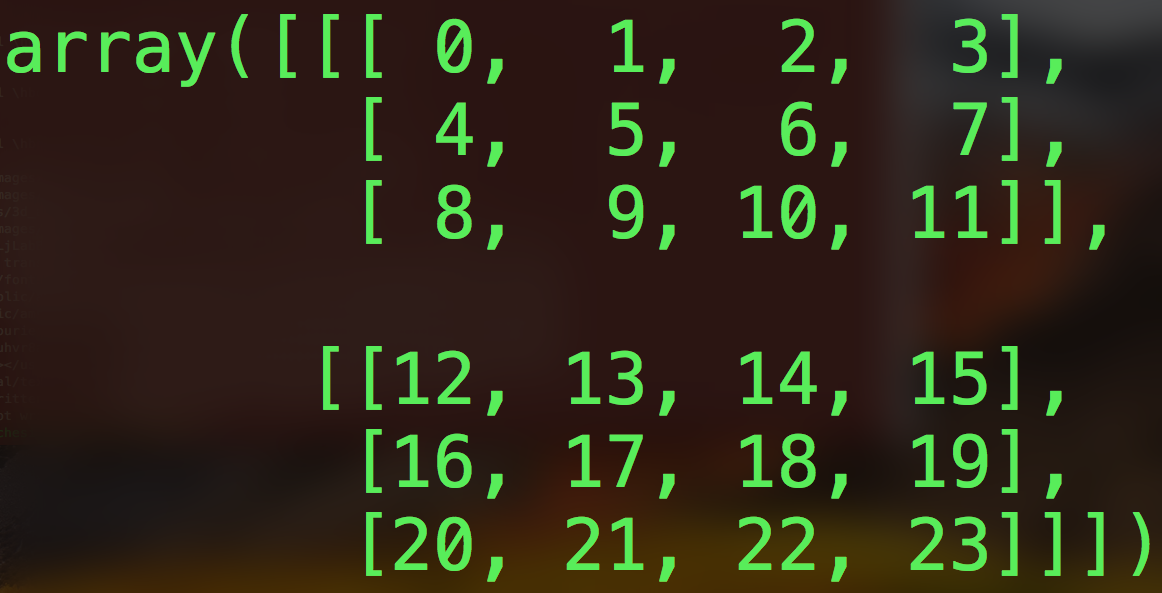
\includegraphics[width=0.65\textwidth]{./images/3d_array_print}
% \caption{
% Visualization of 3D arrays PRINTS.
% }
\label{fig:3d_array_print}
\end{figure}

\newpage
\section{PANDAS}

\vspace{\baselineskip}
\texttt{axis=0} (default) represents rows.
\newline
\texttt{axis=1} represents columns.
\newline

Read / Write:
\begin{easylist}[itemize]
\ListProperties(Style*=$\bullet$ , FinalMark={)})
& \texttt{df.to\char`_csv(\textquotesingle filename.csv\textquotesingle )} ~-- write to a CSV file.
& \texttt{pd.read\char`_csv(\textquotesingle filename.csv\textquotesingle )} ~-- read from a CSV file.
\end{easylist}
\vspace{\baselineskip}

Object Creation:
\begin{easylist}[itemize]
\ListProperties(Style*=$\bullet$ , FinalMark={)})
& \texttt{s = pd.Series([1, 2, 3, 4])} ~-- create a Series (1D).
& \texttt{s = pd.Series([1, 2, 3, 4], index=[\textquotesingle v01\textquotesingle , \textquotesingle v02\textquotesingle , \textquotesingle v03\textquotesingle , \textquotesingle v04\textquotesingle ])}
& \texttt{df = pd.DataFrame([[1,2,3],[4,5,6]])} ~-- create a DataFrame (2D).
& \texttt{df = pd.DataFrame(np.random.randn(2,3), index=[\textquotesingle v01\textquotesingle , \textquotesingle v02\textquotesingle ], columns=[\textquotesingle A\textquotesingle , \textquotesingle B\textquotesingle, \textquotesingle C\textquotesingle])}
& \texttt{df = pd.DataFrame(\{\textquotesingle A\textquotesingle :[33,22,11], \textquotesingle B\textquotesingle :[\textquotesingle baa\textquotesingle , \textquotesingle moo\textquotesingle , \textquotesingle grr\textquotesingle ]\}) }
\end{easylist}

Viewing Data:
\begin{easylist}[itemize]
\ListProperties(Style*=$\bullet$ , FinalMark={)})
& \texttt{df} ~-- top and tails the DataFrame.
& \texttt{df.head()} ~-- typical head.
& \texttt{df.tail(10)} ~-- typical tail.
& \texttt{df.index} ~-- get DataFrame index object.
& \texttt{df.columns} ~-- get DataFrame columns object.
& \texttt{df.shape} ~-- get shape of DataFrame.
& \texttt{df.size} ~-- get number of DataFrame elements.
& \texttt{df.dtypes} ~-- get the data types of the columns.
& \texttt{df.A.unique()} ~-- get the unique entries for a given column.
& \texttt{df.describe()} ~-- provides a basic statistical summary.
& \texttt{df.T} ~-- transpose the DataFrame.
& \texttt{df.to\char`_numpy()} ~-- convert DataFrame to a Numpy array.
& \texttt{df.sort\char`_index(axis=1)} ~-- sort by axis (columns).
& \texttt{df.sort\char`_index(ascending=False)} ~-- sort by axis (rows).
& \texttt{df.sort\char`_values(by=\textquotesingle B\textquotesingle)} ~-- sort by values.
\end{easylist}
\vspace{\baselineskip}

Selection:
\begin{easylist}[itemize]
\ListProperties(Style*=$\bullet$ , FinalMark={)})
& \texttt{df.A} ~-- get column A.
& \texttt{df[\textquotesingle A\textquotesingle]} ~-- select column A.
& \texttt{df[20:25]} ~-- select row slice.
& \texttt{df[\textquotesingle A\textquotesingle][20:25]} ~-- select column and row slice.
& \texttt{df.loc[25]} ~-- get row cross section.
& \texttt{df.loc["2015-09-20 10:00:30"]} ~-- as above, if the rows have names.
& \texttt{df.loc[25, [\textquotesingle A\textquotesingle,\textquotesingle B\textquotesingle]]} ~-- get row cross section for specified columns.
& \texttt{df.loc[20:25, [\textquotesingle A\textquotesingle,\textquotesingle B\textquotesingle]]}~-- select row and column slice (endpoints are \textit{included}).
& \texttt{df.loc["2015-09-20 10:00:30":"2015-09-20 10:00:40", :]}
& \texttt{df.loc[25, \textquotesingle A\textquotesingle]} ~-- get a scalar value.
& \texttt{df.at[25, \textquotesingle A\textquotesingle]} ~-- get fast access to a scalar value.
& \texttt{df.iloc[3:5, 0:2]} ~-- as above but \textbf{specifically} using integer indexing.
& \texttt{df.iloc[3:5, :]} ~-- slicing rows explicitly.
& \texttt{df.iloc[:, 0:2]} ~-- slicing columns explicitly.
& \texttt{df.iat[25, 10]} ~-- as above but \textbf{specifically} using integer indexing.
\end{easylist}
\vspace{\baselineskip}

Boolean Indexing:
\begin{easylist}[itemize]
\ListProperties(Style*=$\bullet$ , FinalMark={)})
& \texttt{df[df.A > 0]} ~-- use a column's values to select data.
& \texttt{df[df.A > 0.5 * (df.B + df.C)]} ~-- \textit{another example}.
& \texttt{df[(df.A > 50) \& (df.B > 50)]} ~-- and \textit{another example}.
& \texttt{df[df > 1.0]} ~-- select values from a DataFrame where a boolean condition is met.
& \texttt{(df > 1.0).sum()} ~-- \textit{little trick which combines techniques}.
& \texttt{df.isin([11,22,33,\textquotesingle C\textquotesingle,\textquotesingle M\textquotesingle,\textquotesingle S\textquotesingle])} ~-- take note of the \textit{isin()} method.
\end{easylist}

\newpage
Setting:
\begin{easylist}[itemize]
\ListProperties(Style*=$\bullet$ , FinalMark={)})
& \texttt{df[\textquotesingle Z\textquotesingle] = [3, 2, 6, 4]} ~-- setting a new column.
& \texttt{df[\textquotesingle Z\textquotesingle] = s} ~~-- NOTE if you use a Series, it doesn't have to be a perfect fit.
& \texttt{df.at[7, \textquotesingle C\textquotesingle] = 888 } -- set scalar values by label.
& \texttt{df.iat[7, 3] = 888 } -- set scalar values by index.
& \texttt{df.loc[:, \textquotesingle D\textquotesingle] = np.array([5] * len(df))} -- set multiple values.
& \texttt{df = df + 2 } ~-- operate on every DataFrame element.
& \texttt{df = df1 + df2 } ~-- \textit{another example}.
& \texttt{df[df < 0] = -df } ~-- can also set values using a boolean mask.
& \texttt{df[\textquotesingle A\textquotesingle] *= -1 } ~-- operate on every element in a column.
& \texttt{df[\textquotesingle A\textquotesingle] = 2 * df[\textquotesingle B\textquotesingle] + df[\textquotesingle C\textquotesingle] } ~-- \textit{another example}. Better than df.apply.
& \texttt{df.loc[3] += 55 } ~-- operate on every element in a row.
& \texttt{df.loc[3] = 2 * df.loc[4] + 55} ~-- \textit{another example}.
\end{easylist}

% \vspace{\baselineskip}
Missing Data:
\begin{easylist}[itemize]
\ListProperties(Style*=$\bullet$ , FinalMark={)})
& \texttt{df.dropna()} ~-- drop any rows with missing data.
& \texttt{df.dropna(axis=1)} ~-- drop any columns with missing data.
& \texttt{df.dropna(how=\textquotesingle any\textquotesingle)} ~-- drop row if there is \textbf{any} NaN instance (default).
& \texttt{df.dropna(how=\textquotesingle all\textquotesingle)} ~-- only drop row if \textbf{all} instances are NaN.
& \texttt{df.fillna(value=55)} ~-- fill missing data with a value.
& \texttt{df.isna()} ~-- get boolean mask where values are NaN.
% & \texttt{df.isna().sum()} ~-- \textit{little trick which combines techniques}.
\end{easylist}

Operations:
% Operations in general \textit{exclude} missing data.
\begin{easylist}[itemize]
\ListProperties(Style*=$\bullet$ , FinalMark={)})
& \texttt{df.mean()} ~-- get the mean of each column.
& \texttt{df.mean(axis=1)} ~-- get the mean of each row.
& \texttt{df.sum(), df.cumsum(), df.max()...} ~-- many different operations.
& \texttt{df.A.sum()} ~-- operate on a single column.
& \texttt{df.apply(lambda col: col.max() - col.min())} ~-- apply function    to cols.
& \texttt{df.apply(lambda row: row.A + row.B, axis=1)} ~-- apply function to rows.
\end{easylist}

Merge:
\begin{easylist}[itemize]
\ListProperties(Style*=$\bullet$ , FinalMark={)})
& \texttt{df = pd.concat([df1, df2])} ~-- concatenate DataFrames.
& \texttt{df = pd.concat([df1, df2], ignore\char`_index=True)} ~-- avoids index clash.
& \texttt{df = pd.concat([df1, df2], axis=1)} -- concatenate DataFrames side-by-side.
& \texttt{df1.append(df2.loc[5], ignore\char`_index=True)} ~-- append a new row.
& \texttt{pd.merge(df1, df2, on=\textquotesingle A\textquotesingle)} ~-- merge DataFrames with same column elements.
& \texttt{pd.merge(df1, df2, left\char`_on=\textquotesingle car\textquotesingle, right\char`_on=\textquotesingle vehicle\textquotesingle)}
~-- merge like this when columns have different names.
\end{easylist}

\vspace{\baselineskip}
Group:
\begin{easylist}[itemize]
\ListProperties(Style*=$\bullet$ , FinalMark={)})
& \texttt{df.groupby(\textquotesingle A\textquotesingle).max()}
~-- for all sets of rows with common column `A'~values,
perform function on all remaining columns.
& \texttt{df.groupby([\textquotesingle A\textquotesingle, \textquotesingle B\textquotesingle]).max()}
~-- like above, but group by both column `A'~and then column `B'.
\end{easylist}

\vspace{\baselineskip}
Time Series:
\begin{easylist}[itemize]
\ListProperties(Style*=$\bullet$ , FinalMark={)})
& \texttt{rng = pd.date\char`_range(\textquotesingle2015-09-20 10:00:00\textquotesingle,\newline .....................periods=100, freq=\textquotesingle S\textquotesingle)} -- creates datetime index.
& \texttt{rng = pd.date\char`_range(start=\textquotesingle2015-09-20 10:00:00\textquotesingle,\newline ....................end=\textquotesingle2019-07-10 17:30:00\textquotesingle, periods=100)} %~-- alternative method.
& \texttt{rng[90].year, rng[90].second} ~-- pull the specific numbers of a given date.
& \texttt{(rng[90] - rng[0]).days} ~-- calculate differences between dates.
& \texttt{df=pd.DataFrame(np.random.rand(100,3), index=rng, columns=list(\textquotesingle ABC\textquotesingle))} ~-- use datetime as a DataFrame index.
\end{easylist}

\vspace{\baselineskip}
Plotting:
\begin{easylist}[itemize]
\ListProperties(Style*=$\bullet$ , FinalMark={)})
& \texttt{df.plot()} ~-- creates graphs from DataFrame.
% & \texttt{df.A.plot()} ~-- \textit{another example}.
& \texttt{df.plot(kind=\textquotesingle scatter\textquotesingle, x=\textquotesingle A\textquotesingle, y=\textquotesingle B\textquotesingle)} ~-- \textit{another example}.
& \texttt{df.hist(bins=50)} ~-- creates histograms from DataFrame.
& \texttt{df.hist(column=\textquotesingle A\textquotesingle, bins=50)} ~-- \textit{another example}.
& \texttt{pd.plotting.scatter\char`_matrix(df[[\textquotesingle A\textquotesingle, \textquotesingle B\textquotesingle, \textquotesingle C\textquotesingle]])} ~-- scatter matrix plot.
\end{easylist}

\newpage
Miscellaneous:
\begin{easylist}[itemize]
\ListProperties(Style*=$\bullet$ , FinalMark={)})
& \texttt{df.drop(\textquotesingle A\textquotesingle, axis=1)} ~-- drop column.
& \texttt{df.drop([\textquotesingle A\textquotesingle, \textquotesingle B\textquotesingle], axis=1)} ~-- drop columns.
& \texttt{df.reindex(columns=[\textquotesingle D\textquotesingle, \textquotesingle A\textquotesingle, \textquotesingle B\textquotesingle])} ~-- select and order columns.
& \texttt{df.rename({\textquotesingle a\textquotesingle:\textquotesingle X\textquotesingle, \textquotesingle b\textquotesingle:\textquotesingle Y\textquotesingle}, axis=1)} ~-- change column names.
& \texttt{df.reset\char`_index(drop=True)} ~-- remove redundancy in indices.
\newline
& \texttt{df.nlargest(10, 'A')} ~-- returns DataFrame ordered by largest column values.
& \texttt{df.nsmallest(20, 'B')} ~-- returns DataFrame ordered by smallest column values.
& \texttt{df.A.value\char`_counts()} ~-- get frequency of column values.
\newline
& \texttt{df.sample(frac = 0.5)} ~-- get fractional random sample from DataFrame.
& \texttt{df.sample(n = 10)} ~-- get nRows random sample from DataFrame.
\end{easylist}

\newpage
\section{SQL}

Creating Tables:\newline
\texttt{DROP TABLE IF EXISTS lut;}\newline
\texttt{CREATE TEMP TABLE lut (code TEXT, full\char`_string TEXT);}\newline
\texttt{INSERT INTO lut VALUES (\textquotesingle inc\textquotesingle, \textquotesingle Included\textquotesingle);}\newline
\texttt{INSERT INTO lut VALUES (\textquotesingle exc\textquotesingle, \textquotesingle Excluded\textquotesingle);}\newline
\texttt{INSERT INTO lut VALUES (\textquotesingle n/a\textquotesingle, \textquotesingle Unspecified\textquotesingle);}

\vspace{\baselineskip}
Manipulating Tables:\newline
\texttt{DELETE FROM lut WHERE code = \textquotesingle n/a\textquotesingle;}\newline
\texttt{ALTER TABLE lut ADD id INT;}\newline
\texttt{UPDATE lut SET id = 1 WHERE code = \textquotesingle inc\textquotesingle;}\newline
\texttt{UPDATE lut SET id = 2 WHERE code = \textquotesingle exc\textquotesingle;}

\vspace{\baselineskip}
Querying Tables:\newline
\texttt{SELECT}\newline
\texttt{*}\newline
\texttt{, weight / (height * height) AS bmi}\newline
\texttt{FROM customers}\newline
\texttt{WHERE has\char`_gp = TRUE}\newline
\texttt{AND weight > 75.0}\newline
\texttt{AND height IS NOT NULL}\newline
\texttt{AND age BETWEEN 16 AND 30}\newline
\texttt{AND eye\char`_colour IN (\textquotesingle blue\textquotesingle, \textquotesingle grey\textquotesingle)}\newline
\texttt{AND name LIKE \textquotesingle B\%\textquotesingle}\newline
\texttt{ORDER BY name}\newline
\texttt{LIMIT 1000}

\vspace{\baselineskip}
Combining Data:\newline
\texttt{SELECT * FROM customers}\newline
\texttt{UNION ALL}\newline
\texttt{SELECT * FROM employees}

\vspace{\baselineskip}
Aggregating Data:\newline
\texttt{SELECT}\newline
\texttt{name}\newline
\texttt{, COUNT(*) AS freq}\newline
\texttt{, MAX(age) AS max\char`_age}\newline
\texttt{, SUM(weight) AS total\char`_weight}\newline
\texttt{, SUM(CASE WHEN age = 18 THEN 1 ELSE 0 END) AS freq\char`_age\char`_18}\newline
\texttt{FROM customers}\newline
\texttt{GROUP BY 1}\newline
\texttt{ORDER BY 1}

\newpage
`IF' Statements:\newline
\texttt{SELECT}\newline
\texttt{>~~~COALESCE(eye\char`_colour, \textquotesingle unknown\textquotesingle) AS eye\char`_colour}\newline
\texttt{>~~~, CASE}\newline
\texttt{>~~~~~~~WHEN age > 65 THEN \textquotesingle OAP\textquotesingle}\newline
\texttt{>~~~~~~~WHEN age > 17 THEN \textquotesingle Adult\textquotesingle}\newline
\texttt{>~~~~~~~ELSE \textquotesingle Child\textquotesingle}\newline
\texttt{>~~~END AS age\char`_cat}\newline
\texttt{FROM customers}

\vspace{\baselineskip}
Inner Joins:\newline
\textit{Returns records that have matching values in both tables.}\newline
\texttt{SELECT}\newline
\texttt{clk.*}\newline
\texttt{, pr.provider\char`_name}\newline
\texttt{FROM holiday.fct\char`_click clk}\newline
\texttt{INNER JOIN common.dim\char`_provider pr USING (provider\char`_id)}

\vspace{\baselineskip}
Left Joins:\newline
\textit{Returns \underline{all} records from the left table (first listed), and the matched records from the right table.}\newline
\texttt{SELECT}\newline
\texttt{*}\newline
\texttt{FROM holiday.fct\char`_click clk}\newline
\texttt{LEFT JOIN common.dim\char`_provider pr ON clk.provider\char`_id = pr.id}

\vspace{\baselineskip}
Full Joins:\newline
\textit{Returns \underline{all} records from the left and right tables.}\newline
\texttt{SELECT}\newline
\texttt{COALESCE(clk.date, bk.date) AS date}\newline
\texttt{, COALESCE(clk.revenue, 0) + COALESCE(bk.revenue, 0) AS revenue}\newline
\texttt{FROM click\char`_revenue clk}\newline
\texttt{FULL OUTER JOIN booking\char`_revenue bk USING (date)}

\vspace{\baselineskip}
The WITH clause is an optional prefix for SELECT:\newline
\texttt{WITH sub\char`_query\char`_1 AS (<INSERT QUERY>),}\newline
\texttt{sub\char`_query\char`_2 AS (<INSERT QUERY>)}\newline\newline
\texttt{SELECT}\newline
\texttt{*}\newline
\texttt{FROM sub\char`_query\char`_1}\newline
\texttt{LEFT JOIN sub\char`_query\char`_2 USING (date)}

\newpage

Window Functions:\newline
\textit{Performs a calculation across a set of table rows that are somehow related to the current row.}

FUNCTION\newline
OVER = using all rows\newline
PARTITION BY = with the same...\newline
ORDER BY = applying function sequentially, ordered by...

\texttt{ROW\char`_NUMBER() OVER (PARTITION BY enq\char`_id ORDER BY sequence) AS risn}

\vspace{\baselineskip}
Creating a local MySQL database from the command line:\newline
\texttt{mysql --host=localhost -u root -p}\newline
\texttt{> create database football\char`_epts;}\newline
\texttt{> show databases;}\newline\newline
\texttt{mysql -u root -p football\char`_epts < session\char`_contexts.sql}\newline
\texttt{mysql -u root -p football\char`_epts < session\char`_files.sql}\newline
\texttt{mysql -u root -p football\char`_epts < session\char`_meta.sql}\newline

\newpage
\section{Statistics}


\textbf{Binomial Distribution}
\newline
A random variable has a binomial distribution if:
\begin{easylist}[itemize]
\ListProperties(Style*=$\bullet$ , FinalMark={)})
\vspace{-2.0mm}
& There are a fixed number of trials, $n$.
\vspace{-3.5mm}
& Each trial has two possible outcomes: success or failure.
\vspace{-3.5mm}
& The probability of success, $p$, is the same for each trial.
\vspace{-3.5mm}
& The trials are independent.
\end{easylist}
\vspace{-5.0mm}
\begin{equation}
P(X=k) = {n \choose k} p^{k} (1-p)^{n-k}
\end{equation}
% 
Where
$n$ is the fixed number of trials,
$k$ is the specified number of successes ($0 \leq k \leq n$),\newline
and $p$ is the probability of success on any given trial.
% 
\begin{easylist}[itemize]
\ListProperties(Style*=$\bullet$ , FinalMark={)})
& The mean of $X$ is $\mu = np$.
\vspace{-3.5mm}
& The standard deviation of $X$ is $\sigma = \sqrt{np(1-p)}$.
\vspace{-3.5mm}
& If $np \geq 10$ and $n(1-p) \geq 10$, you can plug $\mu$ and $\sigma$ into a normal distribution.
\vspace{-3.5mm}
& Note that the raw count, $X$, can be converted into a \underline{proportion} by dividing by $n$.
\end{easylist}

\vspace{+3.5mm}
\textbf{Normal Distribution}
\newline
Probability density function:
\vspace{-5.0mm}
\begin{equation}
f(x) = \frac{1}{\sigma \sqrt{2\pi}} \exp{-\frac{1}{2}\Bigg(\frac{x-\mu}{\sigma}\Bigg)^2}
\end{equation}
% 
making the standarizing substitution
\begin{equation}
z = \frac{x-\mu}{\sigma}
\end{equation}
% 
You get a normal distribution with a mean of zero and standard deviation of unity:
\begin{equation}
f(z) = \frac{1}{\sqrt{2\pi}} \exp{-\frac{1}{2} z^2}
\end{equation}
% 
\begin{equation}
\begin{array}{l}
p(-1 < z < +1) = \int_{-1}^{+1} f(z) \, dz \, = 68.27\%
\\ p(-1.96 < z < +1.96) = \int_{-1.96}^{+1.96} f(z) \, dz \, = 95.00\%
\\ p(-2 < z < +2) = \int_{-2}^{+2} f(z) \, dz \, = 95.45\%
\\ p(-3 < z < +3) = \int_{-3}^{+3} f(z) \, dz \, = 99.73\%
\end{array}
\end{equation}

\vspace{+3.5mm}
\textbf{t- Distribution}
\newline
The t-distribution, with $\nu$ degrees of freedom, has the following probability density function:
% 
\begin{equation}
f_{\nu}(t) = \frac{\Gamma(\frac{\nu + 1}{2})}{\sqrt{\nu \pi} \Gamma(\frac{\nu}{2})} \Big(1 + \frac{t^2}{\nu}\Big)^{-\frac{\nu+1}{2}}
\end{equation}
% 
It has a wider distribution than the z-distribution,
however, in the limit $\nu \rightarrow \infty$ it becomes the z-distribution.
The t-distribution is typically used when analyzing the mean of a population.

\vspace{+3.5mm}
\textbf{Central Limit Theorem}
\newline
% Variability in a population is measured in standard deviations.
Sample means vary because you are only sampling a subset of the whole population.\newline
This variability is measured by the \textit{standard error}.
The standard error of the sample mean is
$\sigma_{\bar{x}} = \sigma_{x} / \sqrt{n}$,
where $\sigma_{x}$ is the population standard deviation and $n$ is the sample size.

If you take a sample of a random variable, $x$,
the \textbf{mean} of this sample, $\bar{x}$, is normally distributed:
\vspace{-10mm}
\begin{enumerate}
\item
If $x$ has a normal distribution.
\item
\vspace{-3mm}
If the sample size is large enough $(n > 30)$,
regardless of the distribution of $x$.\newline
$\rightarrow$ This is the Central Limit Theorem.
\end{enumerate}
%
\vspace{-3.5mm}
The z-score is as follows:
\begin{equation}
z = \frac{\bar{x}-\mu_{\bar{x}}}{\sigma_{\bar{x}}} = \frac{\bar{x}-\mu_x}{\sigma_x / \sqrt{n}} 
\end{equation}


\vspace{+3.5mm}
\textbf{Confidence Intervals}
\newline
Statistics (from samples) are used to estimate parameters (belonging to whole populations).
\begin{easylist}[itemize]
\ListProperties(Style*=$\bullet$ , FinalMark={)})
\vspace{-2.0mm}
& Confidence Interval = Statistic $\pm$ Margin-of-error
\vspace{-3.5mm}
& Confidence Level = The probability that this process provides an interval that correctly
$~~~~~~~~~~~~~~~~~~~~~~~~~~~~~~~~~~$ captures the parameter (e.g. for 95\% confidence, $z^{*} = 1.96$).
\vspace{-3.5mm}
& To find the sample size required,
substitute $\mu - x$ for the desired MOE, and solve for $n$.
\end{easylist}

\underline{Population Mean}, when:
\begin{easylist}[itemize]
\ListProperties(Style*=$\bullet$ , FinalMark={)})
\vspace{-2.0mm}
& the population standard deviation, $\sigma$, is known.
\vspace{-3.5mm}
& \textbf{and} $x$ is normally distributed (or $n>30$).
\end{easylist}
% 
\vspace{-5.0mm}
\begin{equation}
\mu_{\textrm{estimate}} = \bar{x} \pm z^{*} \frac{\sigma}{\sqrt{n}}
\end{equation}

\underline{Population Mean}, when:
\begin{easylist}[itemize]
\ListProperties(Style*=$\bullet$ , FinalMark={)})
\vspace{-2.0mm}
& the population standard deviation, $\sigma$, is unknown.
\vspace{-3.5mm}
& \textbf{or} $x$ is not normally distributed, and $n < 30$.
\end{easylist}
% 
\vspace{-5.0mm}
\begin{equation}
\mu_{\textrm{estimate}} = \bar{x} \pm t^{*}_{n-1} \frac{s}{\sqrt{n}}
\end{equation}

\underline{Difference of Two Population Means}, when:
\begin{easylist}[itemize]
\ListProperties(Style*=$\bullet$ , FinalMark={)})
\vspace{-2.0mm}
& the population standard deviations, $\sigma_{1,2,}$, are known.
\vspace{-3.5mm}
& \textbf{and} $x_{1,2}$ are normally distributed (or $n_{1,2}>30$).
\end{easylist}
% 
\vspace{-5.0mm}
\begin{equation}
(\mu_1 - \mu_2)_{\textrm{estimate}} = (\bar{x}_1 - \bar{x}_2) \pm z^{*} \sqrt{\frac{\sigma_1^2}{n_1} + \frac{\sigma_2^2}{n_2}}
\end{equation}

\underline{Difference of Two Population Means}, when:
\begin{easylist}[itemize]
\ListProperties(Style*=$\bullet$ , FinalMark={)})
\vspace{-2.0mm}
& the population standard deviations, $\sigma_{1,2,}$, are unknown.
\vspace{-3.5mm}
& \textbf{or} $x_{1,2}$ are not normally distributed, and $n_{1,2}<30$.
\end{easylist}
% 
\vspace{-5.0mm}
\begin{equation}
(\mu_1 - \mu_2)_{\textrm{estimate}} = (\bar{x}_1 - \bar{x}_2) \pm t_{n_1+n_2-2}^{*} \sqrt{\frac{(n_1-1)s_1^2 + (n_2-1)s_2^2}{n_1+n_2-2}}
\end{equation}

\underline{Population Proportion}, when:
\begin{easylist}[itemize]
\ListProperties(Style*=$\bullet$ , FinalMark={)})
\vspace{-2.0mm}
& $n\hat{p}\geq10$ and $n(1-\hat{p})\geq10$, where $\hat{p}$ is the sample population proportion.
\end{easylist}
% 
\vspace{-5.0mm}
\begin{equation}
p_{\textrm{estimate}} = \hat{p} \pm z^{*} \sqrt{\frac{\hat{p}(1-\hat{p})}{n}}
\end{equation}

\underline{Difference of Two Population Proportions}, when:
\begin{easylist}[itemize]
\ListProperties(Style*=$\bullet$ , FinalMark={)})
\vspace{-2.0mm}
& $n_{1,2}\hat{p}_{1,2}\geq10$ and $n_{1,2}(1-\hat{p}_{1,2})\geq10$.
\end{easylist}
% 
\vspace{-5.0mm}
\begin{equation}
(p_1 - p_2)_{\textrm{estimate}} = (\hat{p}_1 - \hat{p}_2) \pm z^{*} \sqrt{\frac{\hat{p}_1(1-\hat{p}_1)}{n_1}+ \frac{\hat{p}_2(1-\hat{p}_2)}{n_2}}
\end{equation}

\vspace{+3.5mm}
\textbf{Hypothesis Testing}
\newline
A hypothesis test is a statistical procedure that's designed to test a claim (typically about a population parameter).
In general, you assume a claim is true unless you can prove otherwise.
Here is how you do it:
\vspace{-3.5mm}
\begin{enumerate}
\item
\textbf{Set up null and alternative hypotheses.}
\newline
Examples of null hypothesis...~~~~~~~~~~~~~~$H_0$:~$\mu = 5$,~~~$H_0$:~$p_A = p_B$
\newline
Examples of alternative hypothesis...~~~$H_a$:~$\mu \neq 5$,~~~$H_a$:~$p_A < p_B$
\item
\textbf{Collect data via a random sample.}
\item
\textbf{Calculate the test statistic based on the data.}
\newline
We typically use \textit{standard scores} as test statistics.
Here are some examples.

\underline{Population Mean}, when:
\begin{easylist}[itemize]
\ListProperties(Style*=$\bullet$ , FinalMark={)})
\vspace{-2.0mm}
& the population standard deviation, $\sigma$, is known.
\vspace{-3.5mm}
& \textbf{and} $x$ is normally distributed (or $n>30$).
\end{easylist}
% 
\vspace{-5.0mm}
\begin{equation}
z = \frac{\bar{x} - \mu_0}{\sigma / \sqrt{n}}
\end{equation}

\underline{Population Mean}, when:
\begin{easylist}[itemize]
\ListProperties(Style*=$\bullet$ , FinalMark={)})
\vspace{-2.0mm}
& the population standard deviation, $\sigma$, is unknown.
\vspace{-3.5mm}
& \textbf{or} $x$ is not normally distributed, and $n < 30$.
\end{easylist}
% 
\vspace{-5.0mm}
\begin{equation}
t_{n-1} = \frac{\bar{x} - \mu_0}{s / \sqrt{n}}
\end{equation}

\underline{Difference of Two Population Means}, when:
\begin{easylist}[itemize]
\ListProperties(Style*=$\bullet$ , FinalMark={)})
\vspace{-2.0mm}
& the population standard deviations, $\sigma_{1,2,}$, are known.
\vspace{-3.5mm}
& \textbf{and} $x_{1,2}$ are normally distributed (or $n_{1,2}>30$).
\end{easylist}
% 
\vspace{-5.0mm}
\begin{equation}
z = \frac{(\bar{x}_1 - \bar{x}_2) - 0}{\sqrt{\frac{\sigma_1^2}{n_1} + \frac{\sigma_2^2}{n_2}}}
\end{equation}

\underline{Population Proportion}, when:
\begin{easylist}[itemize]
\ListProperties(Style*=$\bullet$ , FinalMark={)})
\vspace{-2.0mm}
& $n\hat{p}\geq10$ and $n(1-\hat{p})\geq10$, where $\hat{p}$ is the sample population proportion.
\end{easylist}
% 
\vspace{-5.0mm}
\begin{equation}
z = \frac{\hat{p}-p_0}{\sqrt{\frac{p_0(1-p_0)}{n}}}
\end{equation}

\underline{Difference of Two Population Proportions}, when:
\begin{easylist}[itemize]
\ListProperties(Style*=$\bullet$ , FinalMark={)})
\vspace{-2.0mm}
& $n_{1,2}\hat{p}_{1,2}\geq10$ and $n_{1,2}(1-\hat{p}_{1,2})\geq10$.
\end{easylist}
% 
\vspace{-5.0mm}
\begin{equation}
z = \frac{(\hat{p}_1-\hat{p}_2)-0}{\sqrt{\hat{p}(1-\hat{p})(\frac{1}{n_1}+\frac{1}{n_2})}}
~~~~~\textrm{where}~~\hat{p} = \frac{c_1 + c_2}{n_1 + n_2}
\end{equation}

\item
\textbf{Find the p-value for your test statistic.}
\item
\textbf{Decide whether or not to reject $H_0$ based on your p-value.}
\end{enumerate}


\newpage
\section{RESOURCES}

CPP:
\newline
\texttt{Accelerated C++} -- where I learnt.

General Python:
\newline
\texttt{http://chryswoods.com/main/courses/} -- where I learnt.
\newline
\texttt{http://www.tutorialspoint.com/python/}
\newline
\texttt{https://docs.python.org/2.7/tutorial/}

Jupyter Notebooks:
\newline
\texttt{https://www.datacamp.com/community/tutorials/tutorial-jupyter-notebook/}

NumPy:
\newline
\texttt{https://www.numpy.org/devdocs/user/quickstart.html}

Pandas:
\newline
\texttt{https://pandas.pydata.org/pandas-docs/stable/index.html}

Matplotlib:
\newline
\texttt{https://matplotlib.org/tutorials/index.html}

ML:
\newline
\texttt{Hands-on Machine Learning with Scikit-Learn, Keras, and TensorFlow}

% More / General:
% \newline
% \texttt{https://github.com/jakevdp/PythonDataScienceHandbook/}

\newpage

\end{document}